\chapter{Event selection} 
\label{ch:selection}

\minitoc

In this chapter the procedure developed to reconstruct and select \decay{\Bp}{\Dsp\phiz} and \decay{\Bp}{\Dsp\Kp\Km} candidates is described. 
In both cases the branching fractions are measured relative to the normalisation channel \decay{\Bp}{\Dsp\Dzb}.
The corresponding selection for the normalisation channel \decay{\Bp}{\Dsp\Dzb} is also described.  


\section{Dataset}

The search for \decay{\Bp}{\Dsp\phiz} and \decay{\Bp}{\Dsp\Kp\Km} decays are performed using the same data sample collected by the \lhcb experiment.
This data sample includes the entire Run I sample and the first two years of the Run II data collection period.
The total integrated luminosity obtained for each year is listed in Table~\ref{tab:lumi}, along with the corresponding centre-of-mass energies. 

%Data taken with the \lhcb experiment in Run 1 (2011 and 2012) and part of Run 2 (2015 and 2016) are used in this analysis. The total integrated luminosity obtained for each year of data taking is listed in Table~\ref{tab:lumi}, along with the corresponding centre-of-mass energies.  

\begin{table}[t]
 \caption{
   The integrated luminosities obtained during the different data taking periods used in this analysis and the corresponding centre-of-mass energies ($\sqrt{s}$).}
\begin{center}\begin{tabular}{ccc}
   \hline
   Year                    & Integrated luminosity (\invfb)  & $\sqrt{s}$ (\tev) \\ 
   \hline
   2011                    & 1.0  &  7 \\
   2012                    & 2.0  &  8 \\
   2015                    & 0.3  & 13 \\
   2016                    & 1.5  & 13 \\
   \hline
 \end{tabular}\end{center}
\label{tab:lumi}
\end{table}


\section{Online selection}

The online event selection is performed by the \lhcb trigger, which consists of a hardware stage, based on information from the calorimeter and muon
systems, followed by a software stage, which reconstructs the full event.
Reconstructed objects are classified into categories when considering their relationship to the various triggers that fired in a given event. 
\begin{itemize}
\item If the interaction caused by a reconstructed object was sufficient to have fired a given trigger then this object is said to be \texttt{TOS} (Triggered on Signal) with respect to that trigger. As such, if the hits that this object caused were removed from the events the trigger would no longer fire. 
\item Conversely, if the object did not cause the trigger to have fired, the object is \texttt{TIS} (Triggered Independently of Signal) with respect to the trigger. In this case, removal of any hits from the object would not affect the trigger decision. 
\item A third category is possible, \texttt{TOB} (Triggered on Both), where both the signal object and another object are required to reach the threshold to fire a trigger. In this situation neither are sufficient to individually fire the trigger, but removing either one of them would prevent the trigger firing. Events in this category are not considered in this analysis.
\end{itemize}

At the hardware trigger stage, the selected candidates are required to be \texttt{TOS} with respect to the hadronic trigger \texttt{L0Hadron}. This ensures the selected candidates were retained due to corresponding deposits in the hadronic calorimeter. Alternatively, candidates are selected if they are \texttt{TIS} with respect to the global hardware trigger \texttt{L0Global}. This allows candidates that have been retained due another highly energetic decay in the same event to contribute. This could be the decay of hadron resulting from the other \bquark quark in a \bquark\bquarkbar pair production. Any of the hardware trigger subsystems can contribute to the \texttt{L0Global} decision.

{\color{Red}
\begin{itemize}
\item Include approximate TIS TOS fractions
\end{itemize}
}

%At the hardware trigger stage, events are required to have a muon with high \pt or a hadron, photon or electron with high transverse energy in the calorimeters. For hadrons, the transverse energy threshold is 3.5\gev. 

The software trigger stage is split into two parts, \hltone and \hlttwo.
The first stage \hltone requires that the the selected candidates are associated with well reconstructed tracks.

At the second software stage, \hlttwo, two different algorithms are used to select candidates for this analysis.
The first one uses a multivariate algorithm~\cite{BBDT} to identify the presence of a secondary vertex that has two, three or four tracks and is displaced from any PV. At least one of these charged particles must have a transverse momentum $\pt > 1.7\gevc$ and be inconsistent with originating from a PV. 
The second algorithm selects $\phiz$ candidates decaying to two charged kaons. Each kaon must have a transverse momentum $\pt > 0.8\gevc$ and be inconsistent with originating from a PV. The invariant mass of the kaon pair must be within $20\mevcc$ of the known \phiz mass~\cite{PDG2016}.
The inclusive \phiz line is used to maximise the selection efficiencies 

{\color{Red}
\begin{itemize}
\item fractions of events added by each category
\end{itemize}
}

\section{Offline selection}

Events passing any trigger requirement are saved to tape for processing offline. The stages of the offline reconstruction are detailed in this section.

\subsection{Selection requirements}

The large offline data samples passing the online trigger selection are habitually processed in a procedure know within \lhcb as \emph{Stripping}. This centrally managed processing builds candidates from tracks and neutral calorimeter objects in each event according to a set of predefined \emph{Stripping Lines}. Each line builds a specific candidate decay, applying a loose set of preselection requirements, including kinematic, geometric and invariant mass selections. 

The candidate \decay{\Bp}{\Dsp\phiz} and \decay{\Bp}{\Dsp\Kp\Km} decays are built using a very similar set of requirements due to the similar topologies of these decays. The normalisation channel, \decay{\Bp}{\Dsp\Dzb} is built similarly, however the difference in lifetime between the \Dzb and \phiz mesons necessitates a slightly different topology. 
{\color{Green}
\begin{itemize}
\item Schematic of the decay topology
\end{itemize}
}

%%%%%%%%%%%%%%%%%%%%%%%%%%%%%%%%%%%%%%%%%%%%%%%%%%%%%%%%%%
\begin{figure}[!h]
    \centering
    \begin{subfigure}[t]{0.4\textwidth}
        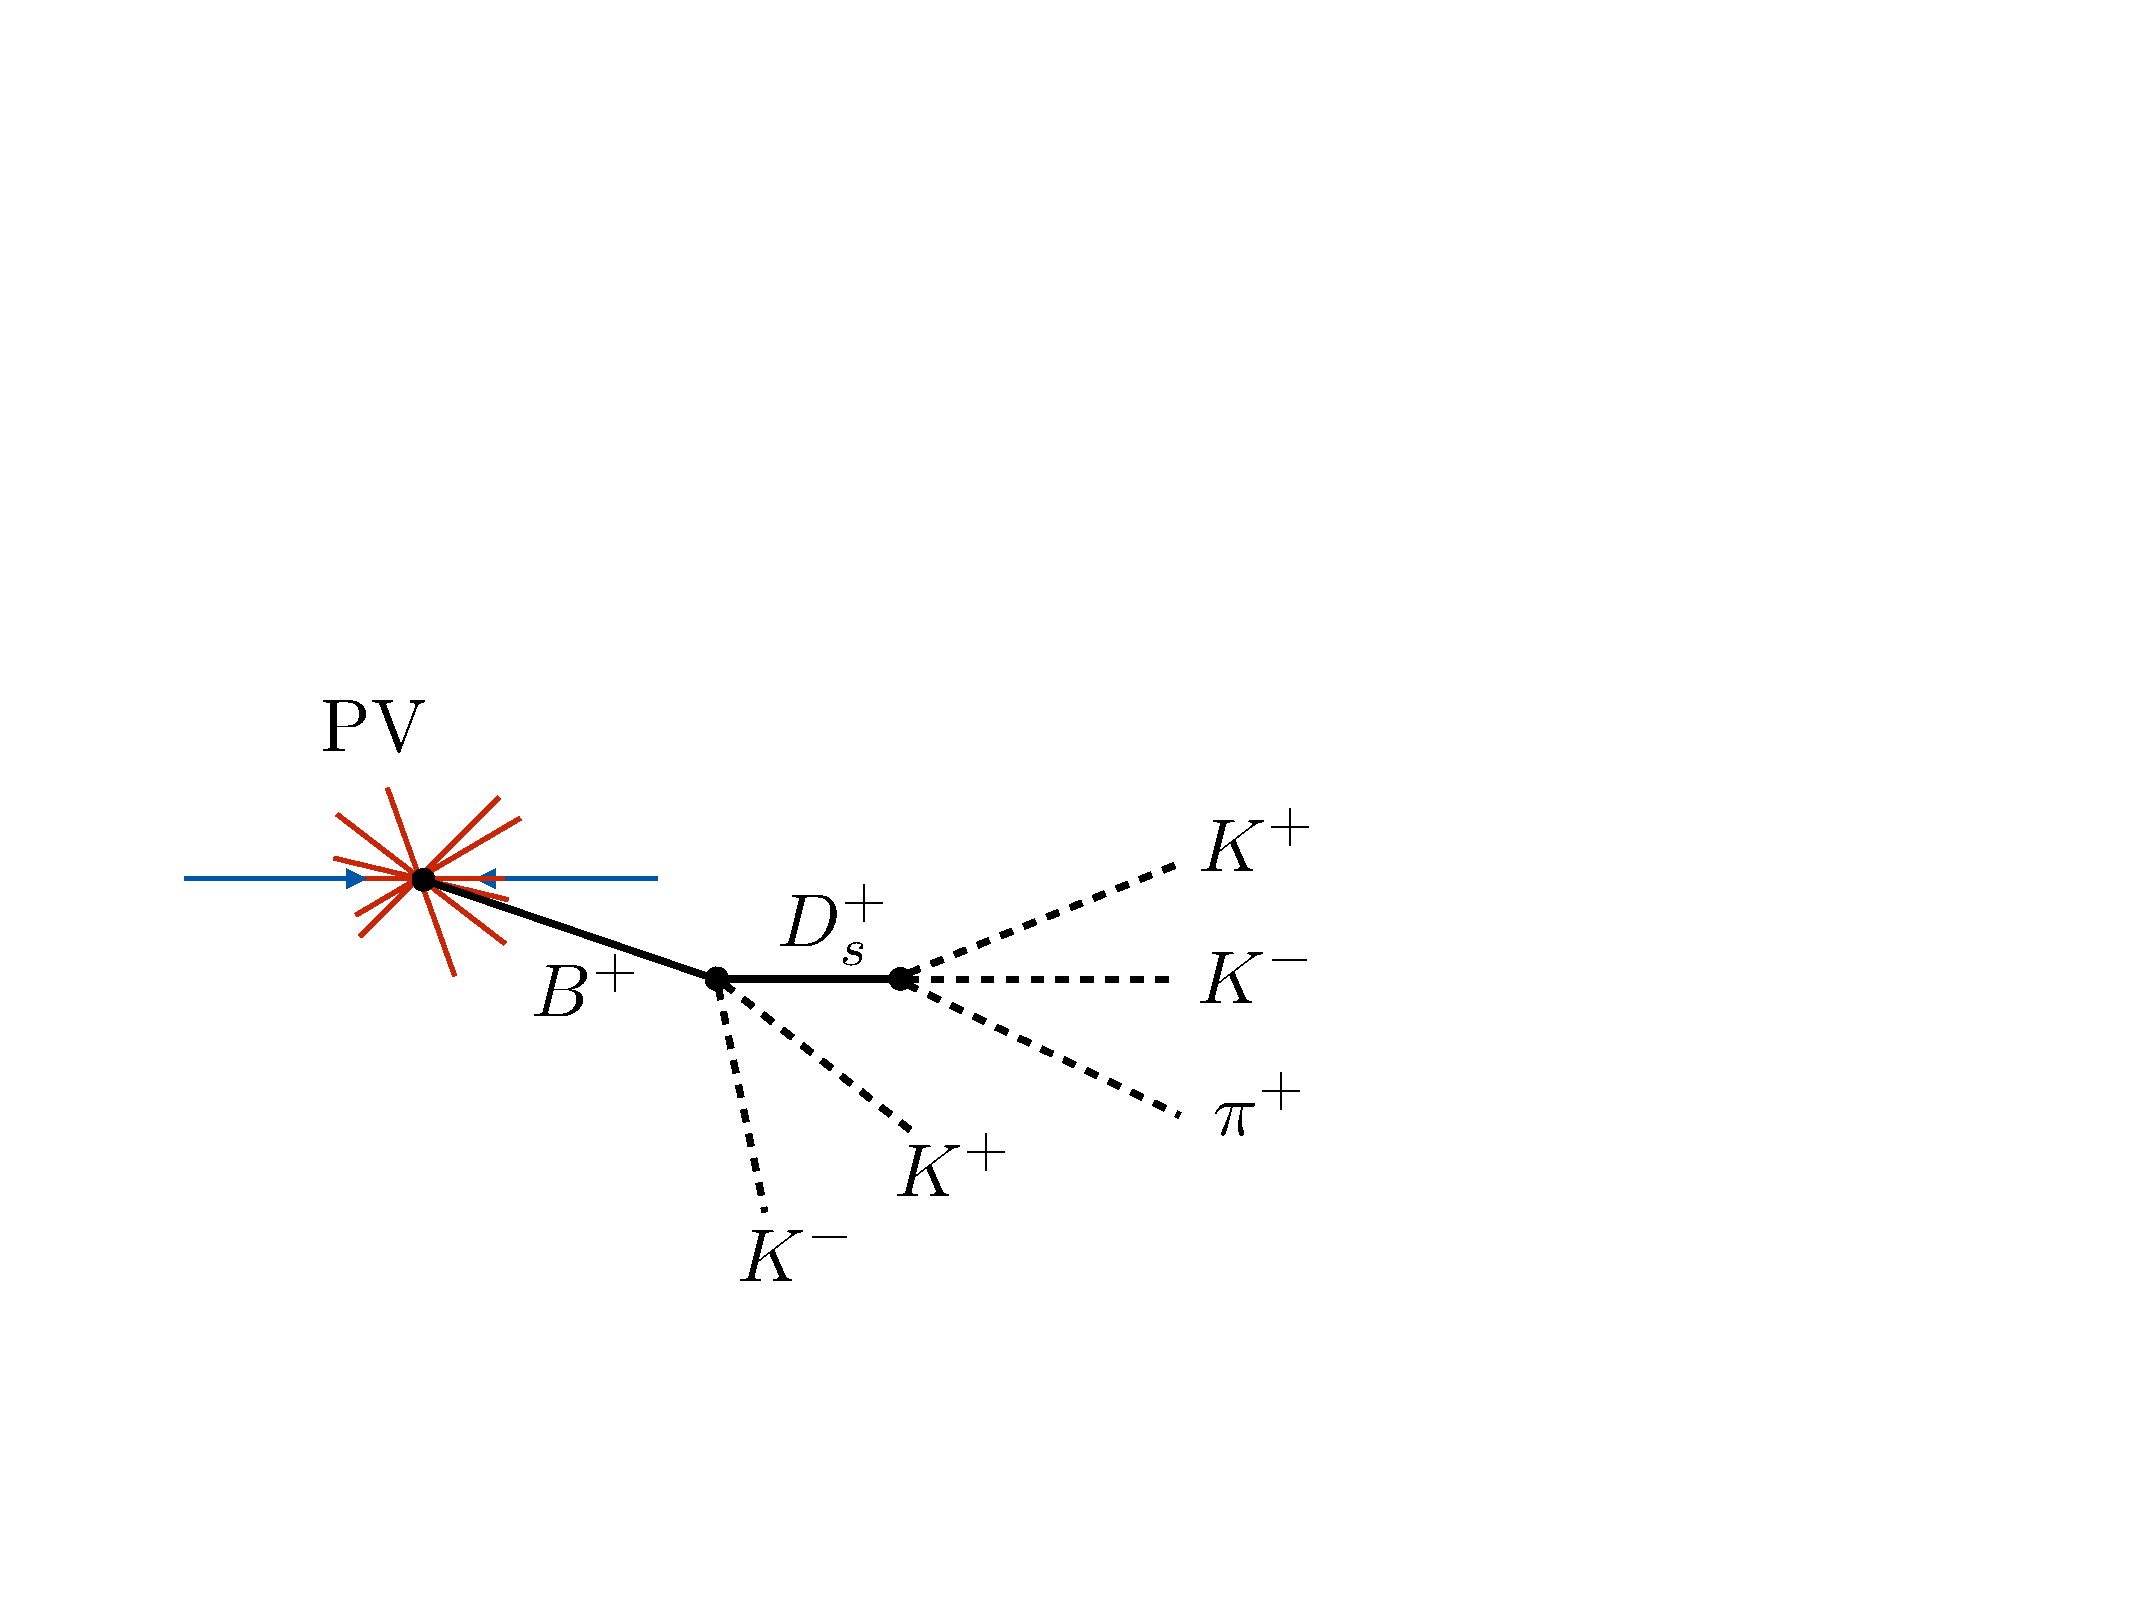
\includegraphics[width=1.0\textwidth]{figs/Selection/B2DsKK_topology.pdf}
        \caption{Signal topology}
    \end{subfigure}%
    \begin{subfigure}[t]{0.4\textwidth}
        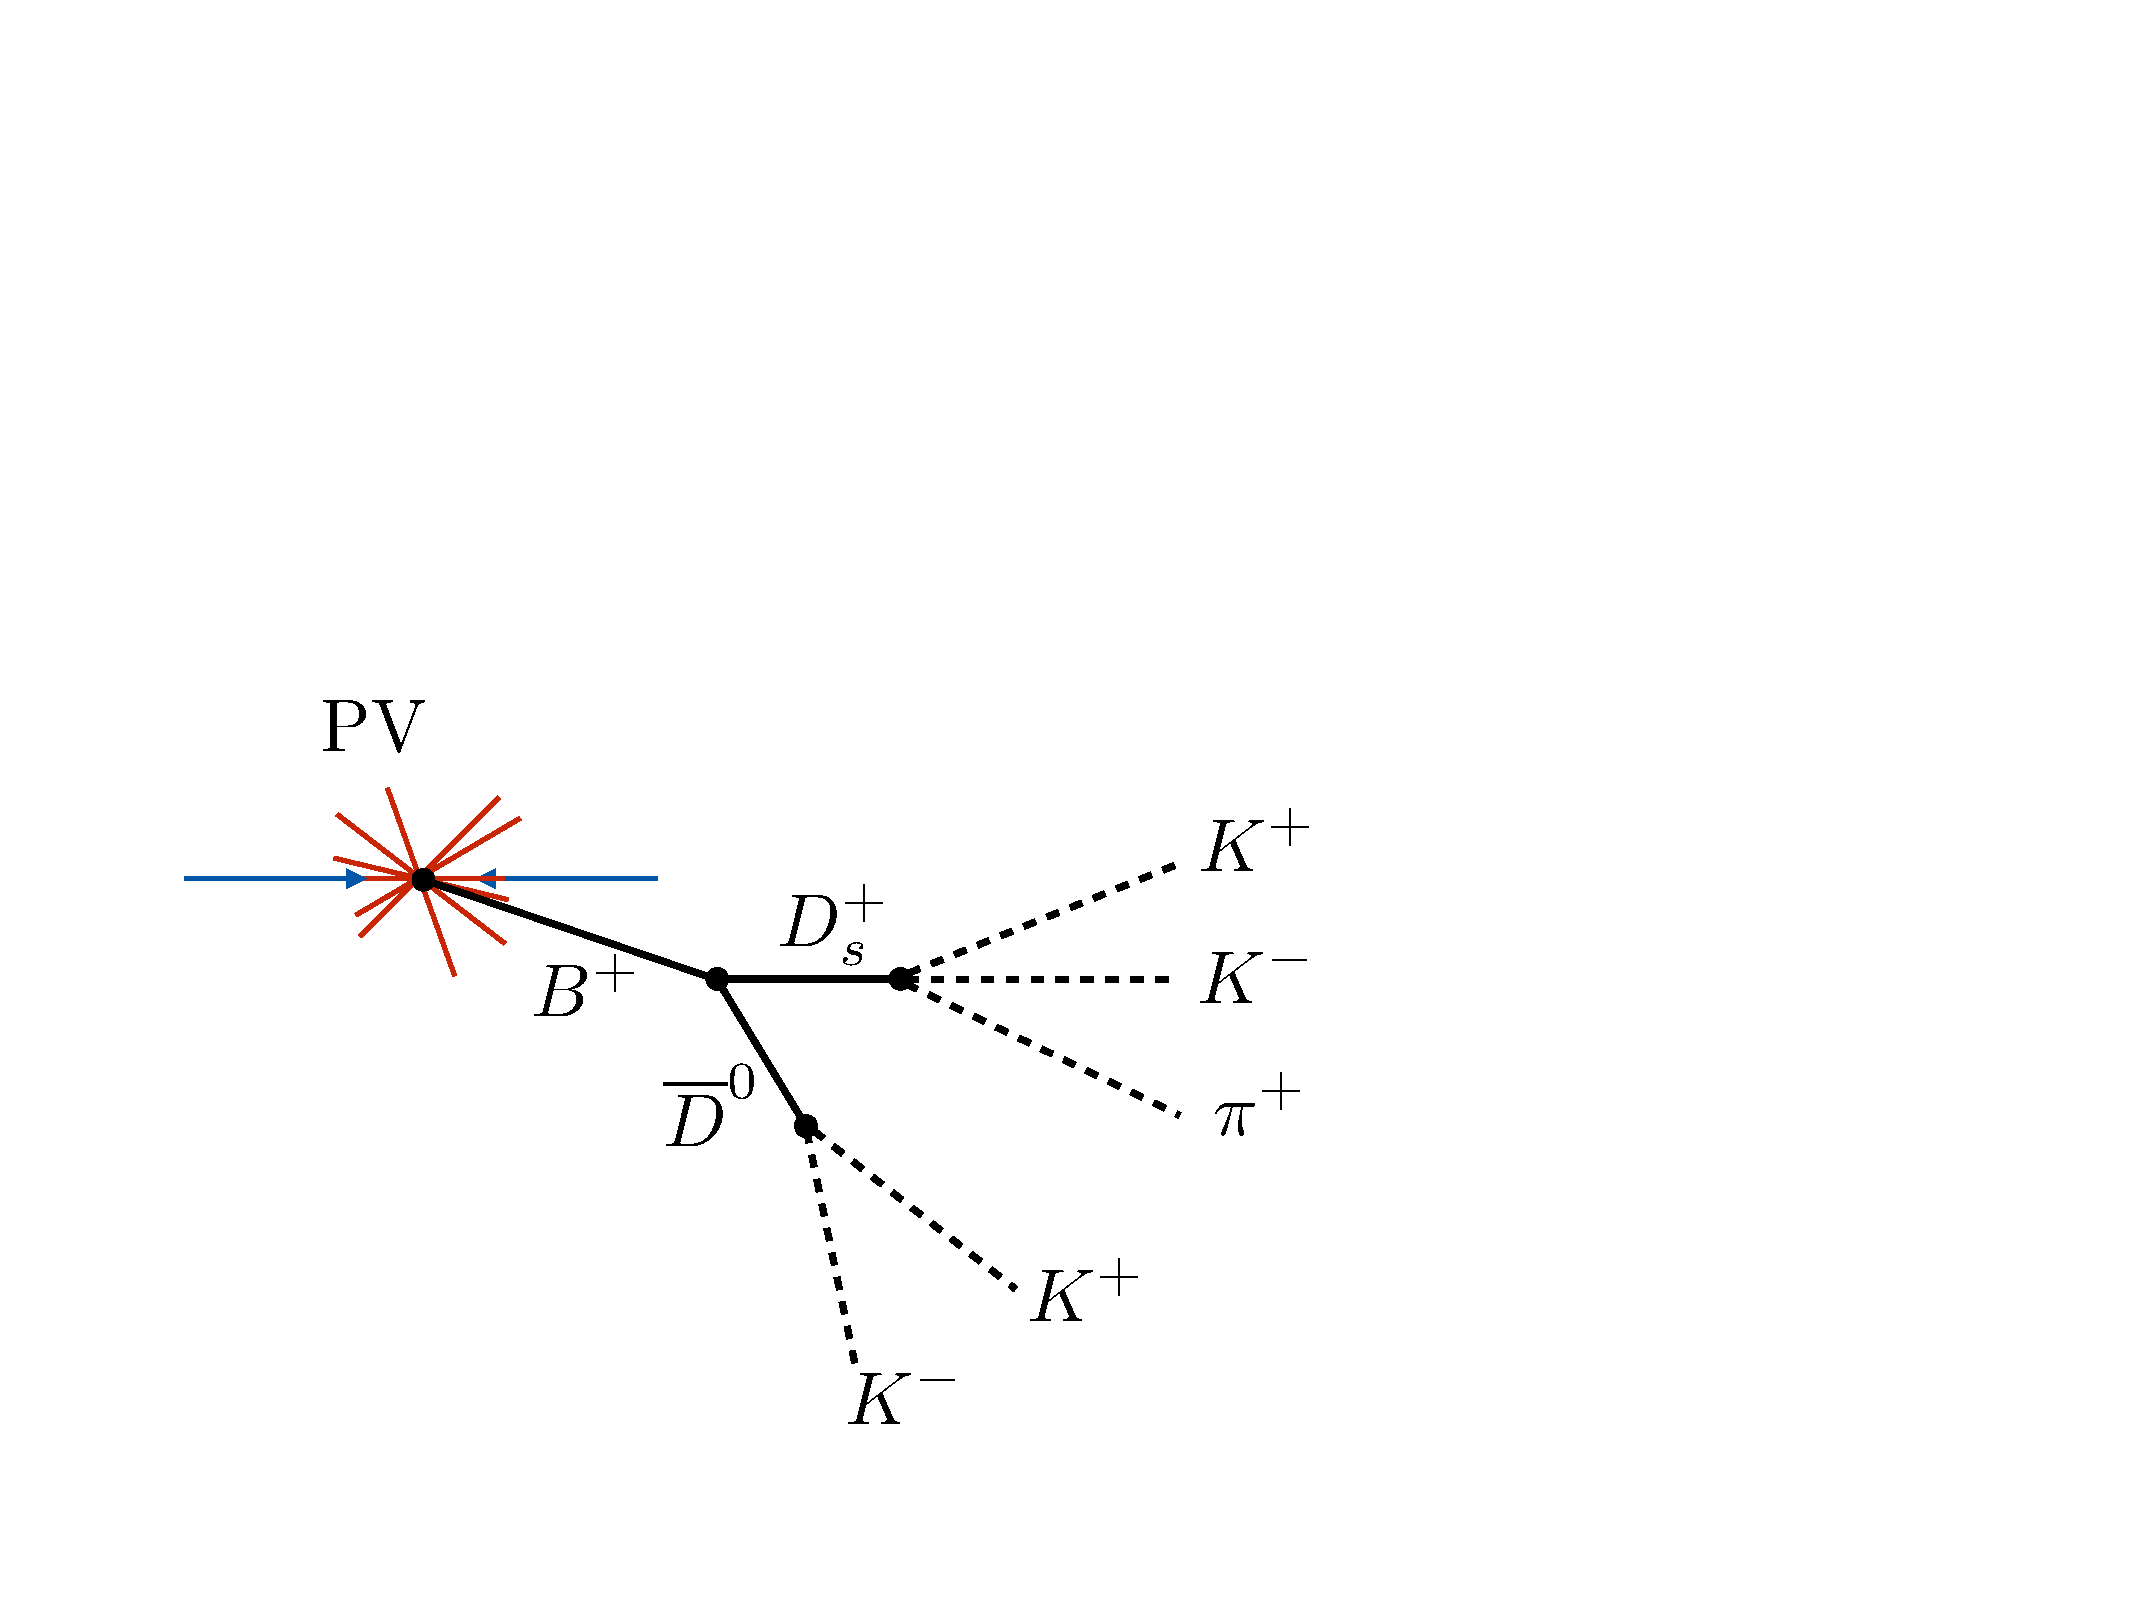
\includegraphics[width=1.0\textwidth]{figs/Selection/B2DsD0_topology.pdf}
        \caption{Normalisation topology}
    \end{subfigure}\\
    \caption{Topologies}
    \label{fig:topo}   
\end{figure}
%%%%%%%%%%%%%%%%%%%%%%%%%%%%%%%%%%%%%%%%%%%%%%%%%%%%%%%%%%


As the final states are fully hadronic the candidates are built from the combination of five tracks. Only \emph{long} tracks (those with hits in the \velo and tracking stations) are used to build these mesons. To ensure these are well reconstructed, the track $\chi^{2}$ per degree of freedom is required to be below $4.0$. Additionally, they are required to have a total momentum $\ptot > 1000 \mevc$ and the projection of the momentum on to the plane transverse to the beam direction is required to be $\pt > 100 \mevc$.
Due to the relatively longlife time of the \Bp and \D mesons, the decay products originate from a vertex that is displaced from the proton-proton collision vertex. Therefore it is possible that the trajectory that the decay products followed didn't pass through the collision position. A requirement is placed on the significance of the impact parameter between the track and the proton-proton collison vertex of $\chi^{2}_{\text{IP}} > 4$ to ensure all of the tracks used are inconsistent with originating at the primary interaction.    
Loose requirements are placed on Particle Identification variables to ensure the tracks are of the required species. These are further tightened as detailed in Section~\ref{sec:pidrequirements}. Incorrect track candidates created by combining unrelated \velo and tracking station stumps are suppressed by requiring the ghost track probability $P_{\text{Ghost}} < 0.4$. 



{\color{Green}
\begin{itemize}
\item Schematic of impact parameter
\end{itemize}
}


%%%%%%%%%%%%%%%%%%%%%%%%%%%%%%%%%%%%%%%%%%%%%%%%%%%%%%%%%%
\begin{figure}[!h]
    \centering
    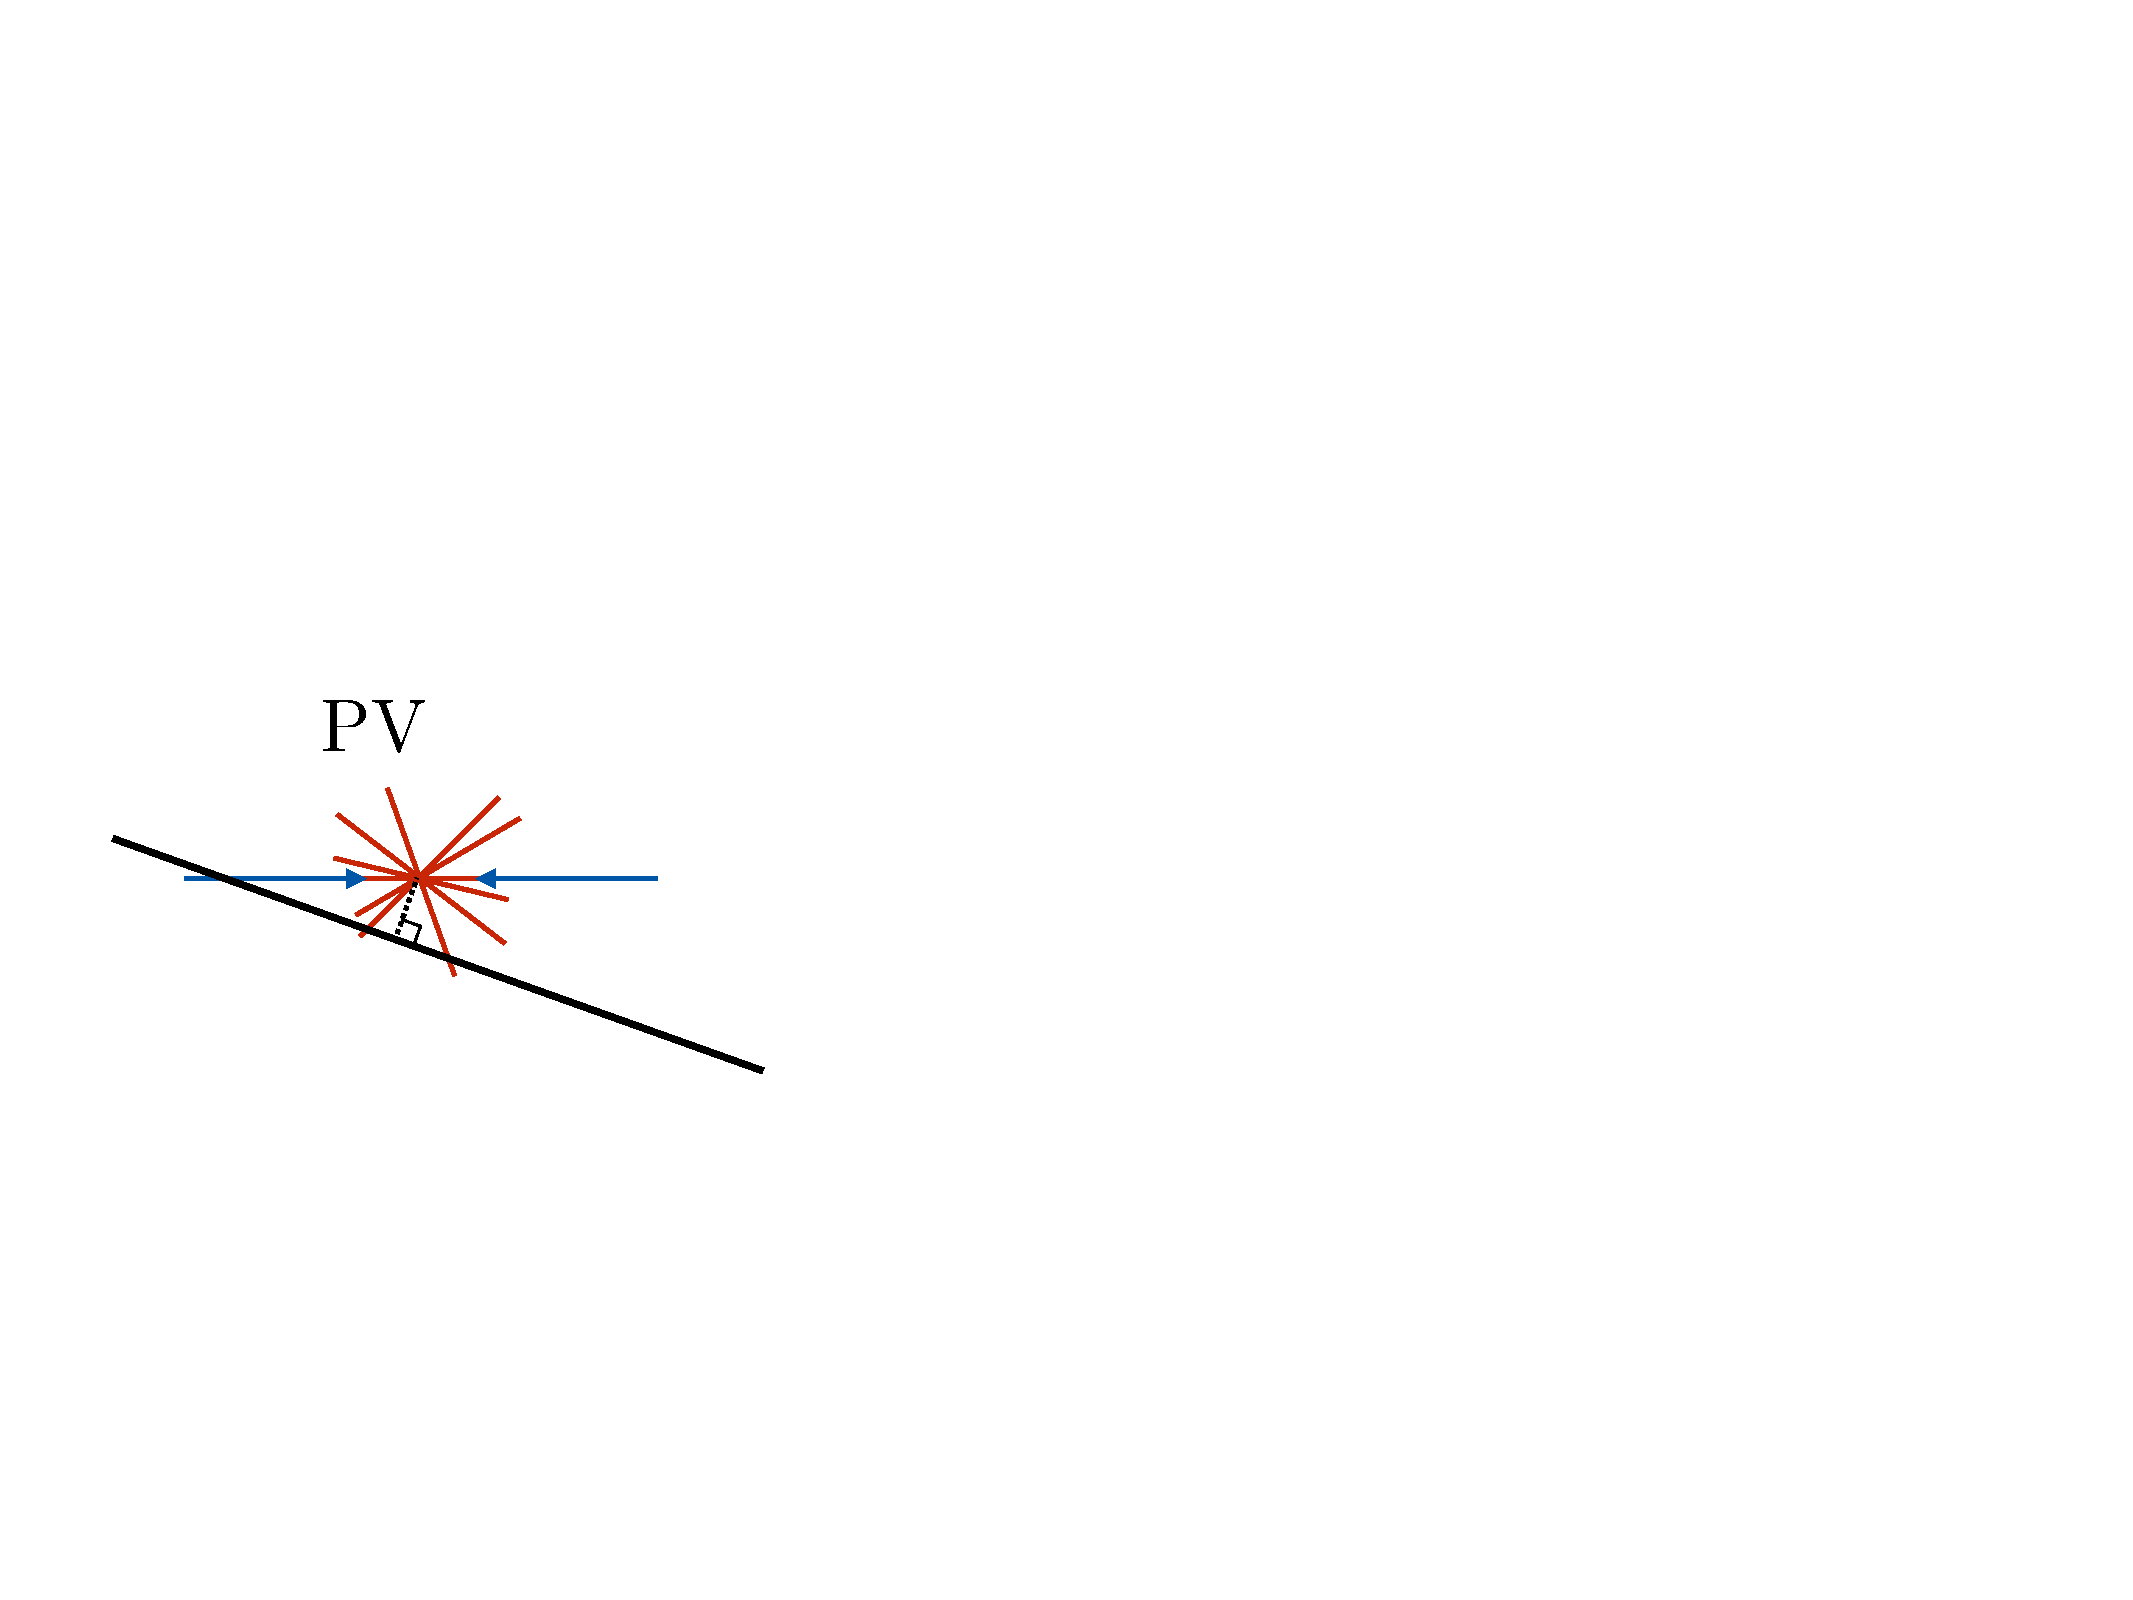
\includegraphics[width=0.4\textwidth]{figs/Selection/Impact_parameter.pdf}
    \caption{Impact parameter}
    \label{fig:topo}   
\end{figure}
%%%%%%%%%%%%%%%%%%%%%%%%%%%%%%%%%%%%%%%%%%%%%%%%%%%%%%%%%%

{\color{Red}
\begin{itemize}
\item Track selection
\item \Dsp and \phiz construction 
\item \Bp construction 
\item diagram of topologies
\item 
\end{itemize}
}




The searches for \decay{\Bp}{\Dsp\phiz} and \decay{\Bp}{\Dsp\Kp\Km} decays employ the use of two different \emph{Stripping Lines} as detailed in Table~\ref{tab:strippinglines}. These differ only in the invariant mass window applied to the $\Kp\Km$ pair used to reconstruct the $\phi$ meson, and in the number of \Dsp decay modes included: the \decay{\Bp}{\Dsp\Kp\Km} line only reconstructs the Cabibbo Favoured (CF) \decay{\Dsp}{\Kp\Km\pip} decay. The \emph{Stripping Line} used to select the normalisation channel \decay{\Bp}{\Dsp\Dzb} is also included in Table~\ref{tab:strippinglines}. This has slightly different requirements allowing the \Dzb meson decay vertex to be be displaced from the \Bp meson decay vertex.


\begin{table}[t]
\caption{Stripping lines used in this analysis.}
\begin{center}
\begin{tabular}{l l}

\hline
Mode & Stripping line \\ 
\hline
\decay{\Bp}{\Dsp\phiz}        & \texttt{StrippingB2DPhiD2HHHPIDBeauty2CharmLine}    \\
\decay{\Bp}{\Dsp\Kp\Km}       & \texttt{StrippingB2DKKD2HHHCFPIDBeauty2CharmLine}   \\
\decay{\Bp}{\Dsp\Dzb}         & \texttt{StrippingB2D0DBeauty2CharmLine}             \\
\hline
\end{tabular}
\end{center}
\label{tab:strippinglines}
\end{table}


The selection requirements imposed on candidate \decay{\Bp}{\Dsp\phiz} and \decay{\Bp}{\Dsp\Kp\Km} decays in their respective \emph{Stripping Lines} is detailed in Table~\ref{tab:strippinglinecuts}. The definitions of the relevant quantities are as follows:
\begin{description}
\item \textbf{Mass:} Invariant mass of the indicated particles. 
\item \textbf{Momentum:} 
\item \textbf{Transverse momentum:} 

\item \textbf{Lifetime:} 

\item \textbf{Products \pt scalar sum:} The sum of the magnitude of the decay products transverse momentum.
\item \textbf{Vertex quality:}

\item \textbf{Impact parameter:} 
\item \textbf{Impact parameter significance:}

\item \textbf{Flight distance significance:} 

\item \textbf{Distance of closest approach:} 
\item \textbf{Ghost track probability:} 
\item \textbf{Direction angle:}

\item \textbf{Particle identification:} 
\end{description}

\begin{table}[h]
\caption{Selection requirements for \decay{\Bp}{\Dsp\phiz} and \decay{\Bp}{\Dsp\Kp\Km} candidates.}
\begin{center}
\begin{tabular}{ l l l}
\hline
Particles      & Quantity                       & Requirement                       \\ 
\hline
\Bp            & Mass                           &  $4750 < m(\Dsp\phiz) < 7000\mevcc$    \\  
%               & Transverse Momentum            &  $\pt > 4000 \gevc$               \\  
               & Products \pt scalar sum        &  $\sum{\pt} > 5000 \mevc$         \\  
               & Vertex quality                 &  $\chi^{2}/N_{\text{DOF}} < 10$   \\  
               & Lifetime                       &  $\tau_{\Bp} > 0.2\ps$            \\  
               & Impact parameter significance  &  $\chi^{2}_{\text{IP}} < 25$      \\  
               & Direction angle                &  $\cos{\theta}>0.999$             \\  
               & \textit{$>$0 decay products with:}    &                                   \\
               & Momentum                       &  $\ptot > 10000 \mevc$            \\  
               & Transverse momentum            &  $\pt > 1700 \mevc$               \\  
               & Impact parameter significance  &  $\chi^{2}_{\text{IP}} > 16$      \\  
               & Impact parameter               &  $\text{IP} > 0.1\mm$             \\  
               & \textit{$>$1 decay products with:}   &                                   \\
               & Momentum                       &  $\ptot > 5000 \mevc$             \\  
               & Transverse momentum            &  $\pt > 500 \mevc$                \\
               &                                &                                   \\  
\Dsp           & Mass                           &  $1770 < m(h^{+}h^{-}h^{+}) < 2068\mevcc$            \\  
               & Products \pt scalar sum        &  $\sum{\pt} > 1800 \mevc$         \\ 
               & Distance of closest approach   &  $\text{DOCA}(h^{+},h^{-}) < 0.5\mm$     \\  
               & Distance of closest approach   &  $\text{DOCA}(h^{+},h^{+}) < 0.5\mm$     \\  
               & Direction angle                &  $\cos{\theta}>0$                 \\  
               & Vertex quality                 &  $\chi^{2}/N_{\text{DOF}} < 10$   \\   
               & Flight distance significance   &  $\chi^{2}_{\text{FD} }  > 36$    \\   
               &                                &                                   \\  
\phiz          & Mass (only for \decay{\Bp}{\Dsp\phiz})&  $|m(\Kp\Km)-m_{\phiz}| < 150\mevcc$\\  
               & Distance of closest approach   &  $\text{DOCA}(\Kp,\Km) < 0.5\mm$  \\  
               & Direction angle                &  $\cos{\theta}>0$                 \\  
               & Vertex quality                 &  $\chi^{2}/N_{\text{DOF}} < 16$   \\   
               & Flight distance significance   &  $\chi^{2}_{\text{FD} }  > 16$    \\   
               &                                &                                   \\  
\Kp (\pip)     & Track quality                  &  $\chi^{2}/N_{\text{DOF}}<4.0$    \\  
               & Transverse momentum            &  $\pt > 100 \mevc$                \\  
               & Momentum                       &  $\ptot > 1000 \mevc$             \\  
               & Impact parameter significance  &  $\chi^{2}_{\text{IP}} > 4$       \\  
               & Ghost track probability        &  $P_{\text{Ghost}} < 0.4$         \\
               & Particle identification        &  $\text{PIDK}<20$ ($\text{PIDK}>-10$)                 \\
%                &                                &                                   \\  
% \Kp            & Particle identification        &  $\text{PIDK}<20$                 \\
%                &                                &                                   \\  
% \pip           & Particle identification        &  $\text{PIDK}>-10$                \\  



\hline
\end{tabular}
\end{center}
\label{tab:strippinglinecuts}
\end{table}

%%%%%%%%%%%%%%%%%%%%%% DONE %%%%%%%%%%%%%%%%%%%%%%
%B CombCut
%(
% ASUM(
%       SUMTREE(
%                PT,(
%                      ISBASIC | 
%                      (ID=='gamma')
%                   )
%                ,0.0
%             )
%       )>5000*MeV) & 
% (AM<7000*MeV) & 
% (AM>4750*MeV)

% B MotherCut

% (VFASPF(VCHI2/VDOF)<10) &
%(BPVLTIME()>0.2*ps) & 
%(BPVIPCHI2()<25) & 
%(BPVDIRA>0.999)
% (INTREE(
%          HASTRACK & 
%          (P>10000*MeV) & 
%          (PT>1700*MeV) & 
%          (TRCHI2DOF<4.) & 
%          (MIPCHI2DV(PRIMARY)>16) & 
%          (MIPDV(PRIMARY)>0.1*mm) )) & 
% (NINTREE(
%          (
%             ISBASIC & 
%             HASTRACK & 
%             (TRCHI2DOF<4.) & 
%             (PT > 500*MeV) & 
%             (P > 5000*MeV)
%          ) > 1
% )


%X2PiPi
%(ASUM(PT)>1000*MeV) & 
% (AM < 5.2*GeV) & 
% (AHASCHILD(
%             (
%                ISBASIC & 
%                HASTRACK & 
%                (TRCHI2DOF<4.) & 
%                (PT > 500*MeV) & 
%                (P > 5000*MeV)
%             )
%          )
% ) & 
% (ADOCA(1,2)<0.5*mm)

%ADMASS('phi(1020)') < 150*MeV

%PiInput
%(TRCHI2DOF<4.0) & 
% (PT>100*MeV) & 
% (P>1000*MeV) & 
% (MIPCHI2DV(PRIMARY)>4.0) & 
% (TRGHP<0.4)


%D2HHHFilter
%
% (NINGENERATION(
%                ('p+'==ABSID) & 
%                (PIDp < -10),1
%                ) == 0
% ) & 
% (NINGENERATION(   
%                ('K+'==ABSID) & 
%                (PIDK < -10)
%                , 1) == 0
% ) & 
% (NINGENERATION(
%                ('pi+'==ABSID) & 
%                (PIDK > 20)
%                , 1) == 0
% )

% D2HHH CombCut
% (ASUM(PT)>1800*MeV) & 
% (in_range(1769.62*MeV,AWM('K+','K+','pi-'),2068.49*MeV)) & 
% (AHASCHILD(
              
%             ISBASIC & 
%             HASTRACK & 
%             (TRCHI2DOF<4.) & 
%             (PT > 500*MeV) & 
%             (P > 5000*MeV)          
%          )
% ) & 
% (ADOCA(1,3)<0.5*mm) & 
% (ADOCA(2,3)<0.5*mm)

% D2HHH MotherCut
% (VFASPF(VCHI2/VDOF)<10) & 
% (BPVVDCHI2>36) & 
% (BPVDIRA>0)

% PhiMotherCut
% (VFASPF(VCHI2/VDOF)<16) & 
% (BPVVDCHI2>16) & 
% (BPVDIRA>0)


%%%%%%%%%%%%%%%%%%%%%%%%%%%%%%%%%%%%%%%%%%%%%%%%%


%HHPionsInput
%(PT>100*MeV) & (P>2000*MeV)


Two slightly different strategies are used for the normalisation channel selection in the search for \decay{\Bp}{\Dsp\phiz} and \decay{\Bp}{\Dsp\Kp\Km} events.
In the former, the dedicated \decay{\Bp}{\Dsp\Dzb} \emph{Stripping Line} listed in Table~\ref{tab:strippinglines} is used to reconstruct the normalisation channel decays.
The \emph{Stripping Line} selection for this line is listed in Table~\ref{tab:strippinglinecuts_norm}.

The \emph{Stripping Line} used in the search for \decay{\Bp}{\Dsp\Kp\Km} decays covers the full $m(\Kp\Km)$ phasespace. This includes the \Dzb mass such that this line reconstructs both the signal and normalisation channels simultaneously. 
Both modes are selected using this line to reduce systematic uncertainty in the ratio of selection efficiencies.

\begin{table}[h]
\caption{Selection requirements for \decay{\Bp}{\Dsp\Dzb} candidates.}
\begin{center}
\begin{tabular}{ l l l}
\hline
Particles      & Quantity                       & Requirement                       \\ 
\hline
\Bp            & Mass                           &  $4750 < m(\Dsp\Dzb) < 7000\mevcc$    \\ 
               & Products \pt scalar sum        &  $\sum{\pt} > 5000 \mevc$         \\  
               & Vertex quality                 &  $\chi^{2}/N_{\text{DOF}} < 10$   \\  
               & Lifetime                       &  $\tau_{\Bp} > 0.2\ps$            \\  
               & Impact parameter significance  &  $\chi^{2}_{\text{IP}} < 25$      \\  
               & Direction angle                &  $\cos{\theta}>0.999$             \\  
               & \textit{$>$0 decay products with:}    &                                   \\
               & Momentum                       &  $\ptot > 10000 \mevc$            \\  
               & Transverse momentum            &  $\pt > 1700 \mevc$               \\  
               & Impact parameter significance  &  $\chi^{2}_{\text{IP}} > 16$      \\  
               & Impact parameter               &  $\text{IP} > 0.1\mm$             \\  
               & \textit{$>$1 decay products with:}   &                                   \\
               & Momentum                       &  $\ptot > 5000 \mevc$             \\  
               & Transverse momentum            &  $\pt > 500 \mevc$                \\
               &                                &                                   \\  
\Dsp           & Mass                           &  $1770 < m(h^{+}h^{-}h^{+}) < 2068\mevcc$            \\  
               & Products \pt scalar sum        &  $\sum{\pt} > 1800 \mevc$         \\ 
               & Distance of closest approach   &  $\text{DOCA}(h^{+},h^{-}) < 0.5\mm$     \\  
               & Distance of closest approach   &  $\text{DOCA}(h^{+},h^{+}) < 0.5\mm$     \\  
               & Direction angle                &  $\cos{\theta}>0$                 \\  
               & Vertex quality                 &  $\chi^{2}/N_{\text{DOF}} < 10$   \\   
               & Flight distance significance   &  $\chi^{2}_{\text{FD} }  > 36$    \\   
               &                                &                                   \\  
\Dzb           & Mass                           &  $1765 < m(h^{+}h^{-}h^{+}) < 1965\mevcc$\\  
               & Distance of closest approach   &  $\text{DOCA}(\Kp,\Km) < 0.5\mm$  \\  
               & Direction angle                &  $\cos{\theta}>0$                 \\  
               & Vertex quality                 &  $\chi^{2}/N_{\text{DOF}} < 10$   \\   
               & Flight distance significance   &  $\chi^{2}_{\text{FD} }  > 36$    \\   
               &                                &                                   \\  
\Kp (\pip)     & Track quality                  &  $\chi^{2}/N_{\text{DOF}}<4.0$    \\  
               & Transverse momentum            &  $\pt > 100 \mevc$                \\  
               & Momentum                       &  $\ptot > 1000 \mevc$             \\  
               & Impact parameter significance  &  $\chi^{2}_{\text{IP}} > 4$       \\  
               & Ghost track probability        &  $P_{\text{Ghost}} < 0.4$         \\
               & Particle identification        &  $\text{PIDK}<20$ ($\text{PIDK}>-10$)                 \\
%                &                                &                                   \\  
% \Kp            & Particle identification        &  $\text{PIDK}<20$                 \\
%                &                                &                                   \\  
% \pip           & Particle identification        &  $\text{PIDK}>-10$                \\  





\hline
\end{tabular}
\end{center}
\label{tab:strippinglinecuts_norm}
\end{table}



% D2KKPi Mother
% (VFASPF(VCHI2/VDOF)<10) & (BPVVDCHI2>36) & (BPVDIRA>0)



% D2KKPi Comb12 
% (ADOCA(1,2)<0.5*mm)


% D2KKPi Comb
% 
% (ASUM(PT)>1800*MeV) & 
% (in_range(1769.62*MeV,AWM('K-','K-','pi+'),2068.49*MeV)) & 
% (AHASCHILD(
%             ISBASIC & 
%             HASTRACK & 
%             (TRCHI2DOF<4.) & 
%             (PT > 500*MeV) & 
%             (P > 5000*MeV)  
%          )  
% ) & 
% (ADOCA(1,3)<0.5*mm) & 
% (ADOCA(2,3)<0.5*mm)



% K input 
% (TRCHI2DOF<4.0) & (PT>100*MeV) & (P>1000*MeV) & (MIPCHI2DV(PRIMARY)>4.0) & (TRGHP<0.4)


% D2KK Mother
% 
% (VFASPF(VCHI2/VDOF)<10) & 
% (BPVVDCHI2>36) & 
% (BPVDIRA>0)




% D2KK Comb
% 
% (ASUM(PT)>1800*MeV) & 
% (in_range(1764.84*MeV,AWM('K+','K-'),1964.84*MeV)) & 
% (AHASCHILD(
%          ISBASIC & 
%          HASTRACK & 
%          (TRCHI2DOF<4.) & 
%          (PT > 500*MeV) & 
%          (P > 5000*MeV)    
%       )
% ) & 
% (ADOCA(1,2)<0.5*mm)

% D2HH
% (NINGENERATION(('p+'==ABSID) & (PIDp < -10),1) == 0) & (NINGENERATION(('K+'==ABSID) & (PIDK < -10), 1) == 0) & (NINGENERATION(('pi+'==ABSID) & (PIDK > 20), 1) == 0)


% B mother cut
% (VFASPF(VCHI2/VDOF)<10) & 
% (
%    INTREE(HASTRACK & 
%    (P>10000*MeV) & 
%    (PT>1700*MeV) & 
%    (TRCHI2DOF<4.) & 
%    (MIPCHI2DV(PRIMARY)>16) & 
%    (MIPDV(PRIMARY)>0.1*mm))
% ) & 
% (
%    NINTREE( 
%             ISBASIC & 
%             HASTRACK & 
%             (TRCHI2DOF<4.) & 
%             (PT > 500*MeV) & 
%             (P > 5000*MeV)     
%          ) > 1
% ) & 
% (BPVLTIME()>0.2*ps) & 
% (BPVIPCHI2()<25) & 
% (BPVDIRA>0.999)


% B comb
% (ASUM(
%    SUMTREE(PT,ISBASIC,0.0) )>5000*MeV
% ) & 
% (AM<7000*MeV) & 
% (AM>4750*MeV)

%%%%%%%%%%%%% done %%%%%%%%%%%


\clearpage


\subsection{Particle identification requirements}
\label{sec:pidrequirements}
Particle identification variables help to determine the species of tracks passing though the \lhcb detector. Using information from the RICH sub-detectors, the likelihood of different mass hypotheses are compared to the pion hypothesis. Loose requirements are made on the kaon hypothesis PID variable to reduce the contribution from other types of hadrons and background from other \bquark-hadron decays with misidentified hadrons. 
%For the signal decays, the overall efficiency of the PID requirements varies from 80\% to 90\%, depending on the \Dsp mode.

{\color{Red}
\begin{itemize}
\item Include actual cuts
\item description of what DLLs mean
\end{itemize}
}

\subsection{Charmless and single-charm backgrounds}


Decays of \Bp mesons that didn't proceed via a \D meson could form a peaking background below the invariant mass distributions when they decay to the same final state.
The signal mode could receive contributions from the decays $\decay{\Bp}{h^{+}h^{-}h^{+}\phiz}$ or $\decay{\Bp}{h^{+}h^{-}h^{+}h^{+}h^{-}}$, referred to as charmless backgrounds.
The normalisation mode is also susceptible, however as it involves two charm mesons it could receive contributions from the decays $\decay{\Bp}{h^{+}h^{-}h^{+}\Dzb}$ or $\decay{\Bp}{\Dsp h^{+}h^{-}}$, referred to as single-charm backgrounds, and $\decay{\Bp}{h^{+}h^{-}h^{+} h^{+}h^{-}}$ referred to as a charmless background.
These backgrounds can be suppressed by requiring the \D meson decay vertex to be displaced from the \Bp meson decay vertex. Requirements are applied to the significance of the vertex separation ($\chi^{2}_{\text{FD}}$).

The residual yields of charmless backgrounds in the signal mode are estimated by performing a fit to the \Bp invariant mass for candidates with $25 < |m(h^{+}h^{-}h^{+}) - m(\Dsp)| < 50\mevcc $. This background estimation is performed separately for the \decay{\Bp}{\Dsp\phiz} and \decay{\Bp}{\Dsp\Kp\Km} searches. 

For the \decay{\Bp}{\Dsp\Dzb} normalisation channel, a two-dimensional optimisation is performed to calculate the contribution from decays without a \Dsp meson, \Dzb meson or both. 
The two-dimensional space defined by the \Dsp and \Dzb masses is split into four types of area as shown in Fig~\ref{fig:2d_normalisation}:
\begin{enumerate}
\item Areas in which only $\decay{\Bp}{h^{+}h^{-}h^{+}h^{+}h^{-}}$ decays contribute (red).
\item Areas in which either $\decay{\Bp}{D_{s}^{+}h^{+}h^{-}}$  or $\decay{\Bp}{h^{+}h^{-}h^{+} h^{+}h^{-}}$ decays can contribute (blue). 

\item Areas in which either $\decay{\Bp}{h^{+}h^{-}h^{+}\Dzb}$ or $\decay{\Bp}{h^{+}h^{-}h^{+} h^{+}h^{-}}$ decays can contribute (green). 
\item The signal region in which $\decay{\Bp}{D_{s}^{+} \Dzb}$, $\decay{\Bp}{h^{+}h^{-}h^{+}\Dzb}$, $\decay{\Bp}{D_{s}^{+}h^{+}h^{-}}$ or $\decay{\Bp}{h^{+}h^{-}h^{+}h^{+}h^{-}}$ decays could contribute (black).
\end{enumerate}   

Asymmetric \Dzb sidebands are used to prevent misidentified \decay{\Bp}{\Dsp (\decay{\Dzb}{\Km\pip})} decays from being included in the sideband sample.
The optimal selection requirements are chosen such that the maximal signal efficiency is achieved for a residual charmless contribution of 2\% of the normalisation yield.

%%%%%%%%%%%%%%%%%%%%%%%%%%%%%%%%%%%%%%%%%%%%%%%%%%%%%%%%%%
\begin{figure}[!h]
    \centering
        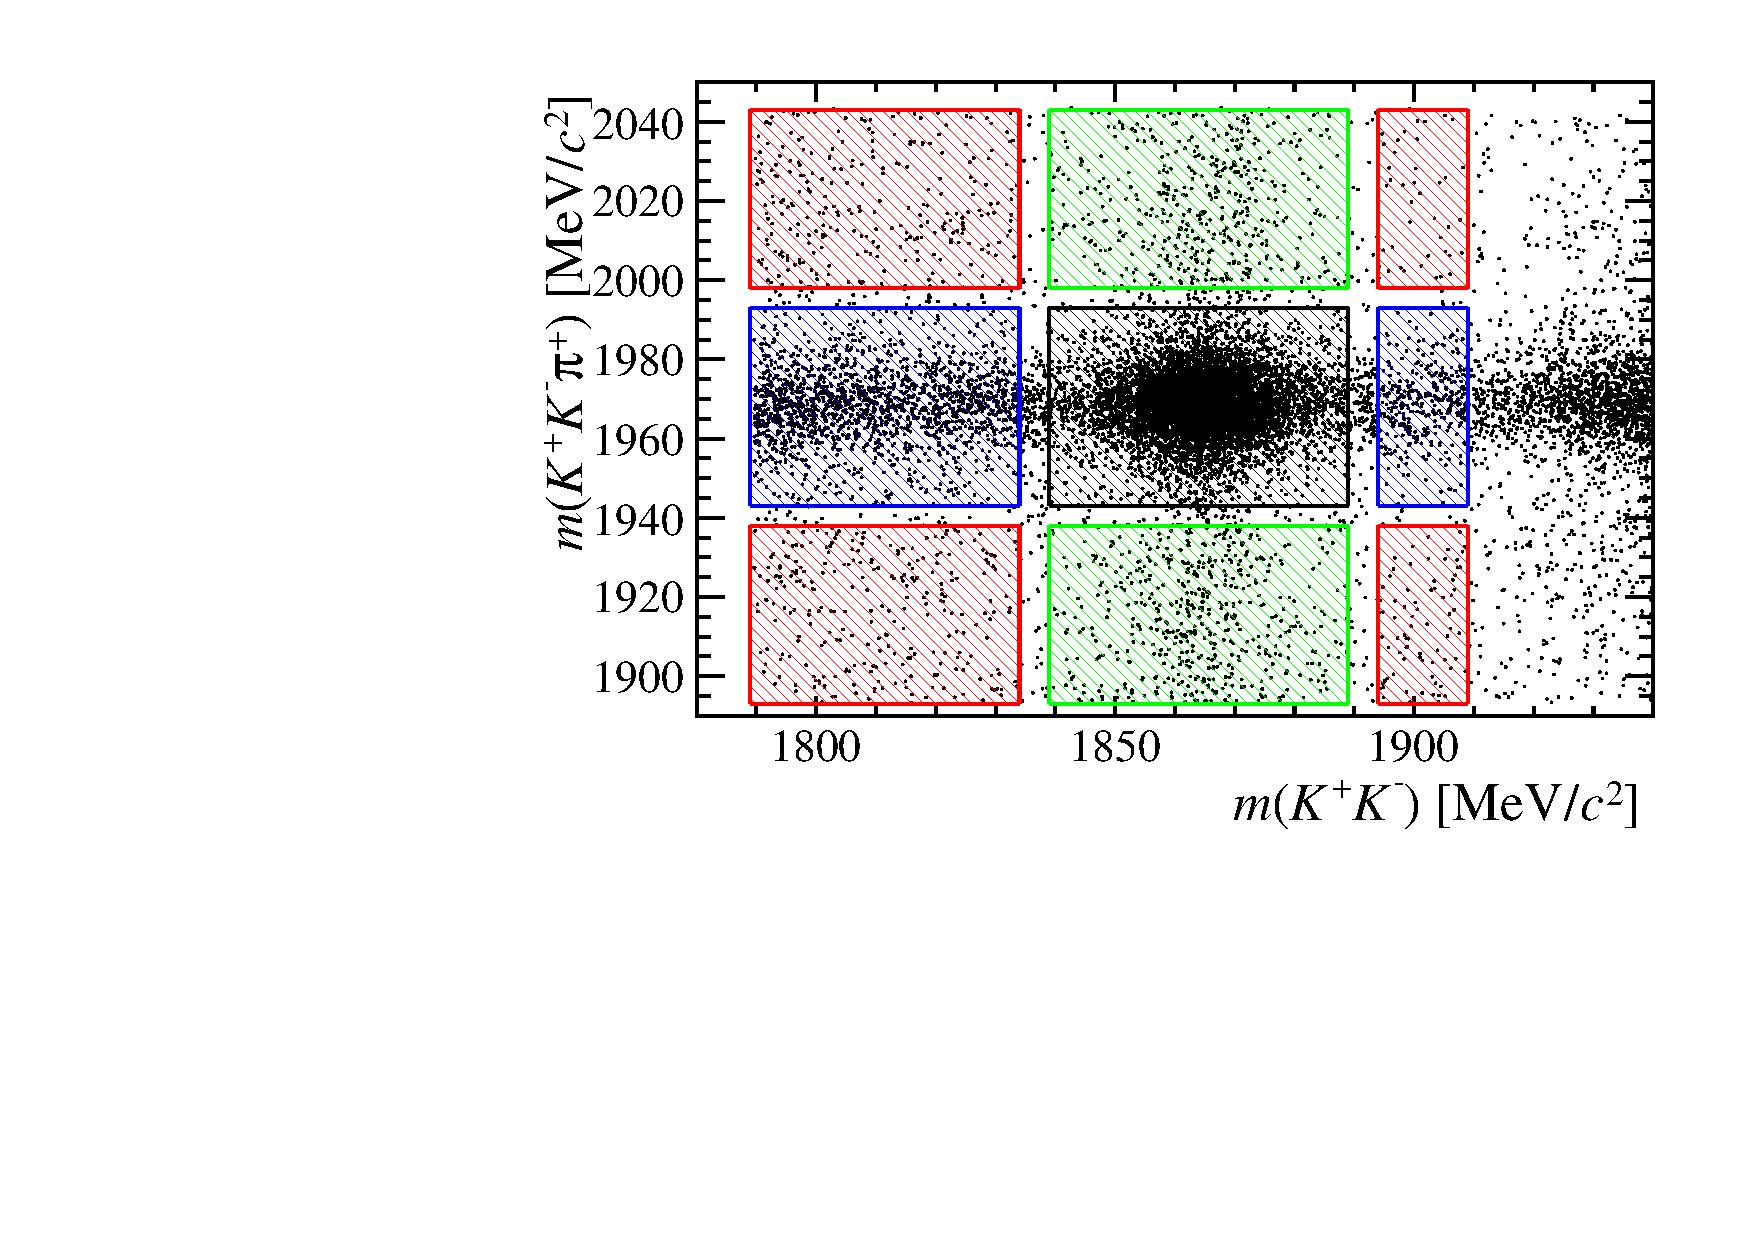
\includegraphics[width=0.6\textwidth]{figs/Selection/B2DsD0_2D_mass_Ds2KKPiRun2.pdf}
        \caption{Two dimensional normalisation}
    \label{fig:2d_normalisation}   
\end{figure}
%%%%%%%%%%%%%%%%%%%%%%%%%%%%%%%%%%%%%%%%%%%%%%%%%%%%%%%%%%


{\color{Red}
\begin{itemize}
\item Optmised separately for \decay{\Bp}{\Dsp\Kp\Km} and \decay{\Bp}{\Dsp\phiz}
\item Include plots of selected cuts
\item include table of expected residual yields 
\end{itemize}
}


\subsection{Misidentified \D and \Lc hadrons}
\label{sec:pidvetos}

It is possible for the samples \Dsp mesons to be contaminated by other misidentified decays of \Dp mesons or \Lc baryons in which one of the decay products has been incorrectly identified.
The invariant mass of the \Dsp meson is recalculated, swapping the mass hypothesis of the ambiguous track to that of the \kaon, or \proton, depending on the decay mode. 
The particle identification requirements are tightened within a mass window around the \Dp or \Lc mass, effectively removing this crossfeed. For the mode \decay{\Dsp}{\Kp\Km\pip}, the vetoes are not applied to candidates for which $m|(\Km\Kp)-m_{\phiz}| < 10\mevcc$ as there are a high purity of \decay{\Dsp}{\Kp\Km\pip} decays in this region.

The specific vetoes included in this selection are listed in Table~\ref{table:pidvetos}. 

\begin{table*}[!ht]
\begin{center}
\begin{tabular}{ l l l }
\hline
Decay Mode & Misidentified decay\\
\hline
\decay{\Dsp}{{\color{Red}\Kp}\Km\pip}   & \decay{\Dp}{{\color{Red}\pip}\Km\pip}    \\
                           & \decay{\Lc}{{\color{Red}\Pp}\Km\pip}     \\
                           &                             \\
\decay{\Dsp}{{\color{Red}\Kp}\pim\pip}  & \decay{\Dp}{{\color{Red}\pip}\pim\pip}   \\
                           &                             \\

\hline
\end{tabular}
\caption{Misidentified decays targeted by vetoes. The ambiguous track is highlighted in red in each case.}
\label{table:pidvetos}
\end{center}
\end{table*}


The invariant mass distributions for each the misidentified \decay{\Dsp}{\Kp\Km\pip} decays are shown with and without the MVA requirements in Figs.~\ref{fig:PIDVetos_Ds2KKPi_D_Veto} and \ref{fig:PIDVetos_Ds2KKPi_Lc_Veto} for both the signal \decay{\Bp}{\Dsp\phiz} and normalisation \decay{\Bp}{\Dsp\Dzb} decays.



%%%%%%%%%%%%%%%%%%%%%%%%%%%%%%%%%%%%%%%%%%%%%%%%%%%%%%%%%%
\begin{figure}[!h]
    \centering
    \begin{subfigure}[t]{0.4\textwidth}
        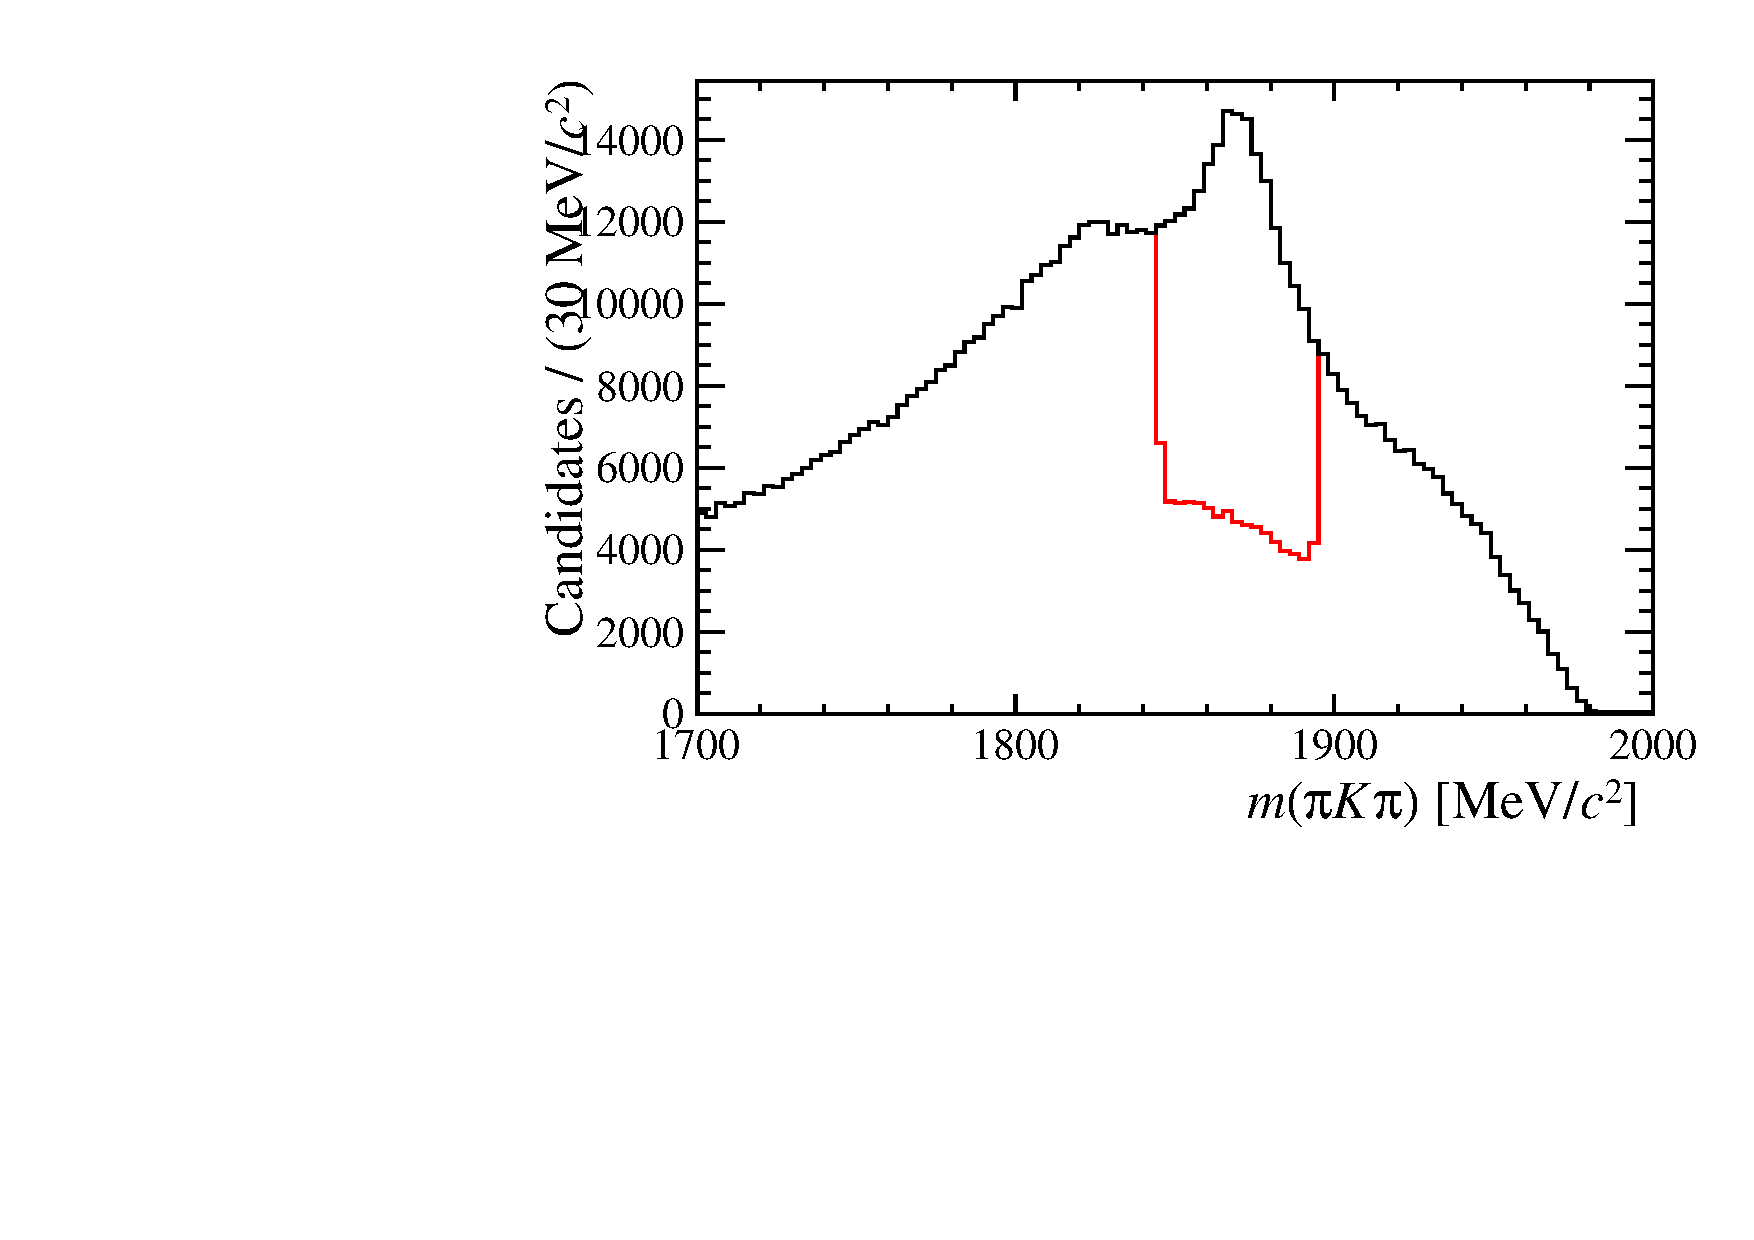
\includegraphics[width=1.0\textwidth]{figs/Selection/B2DsD0_Ds2KKPi_D_Veto_NoBDT.pdf}
        \caption{Normalisation without selection}
    \end{subfigure}%
    \begin{subfigure}[t]{0.4\textwidth}
        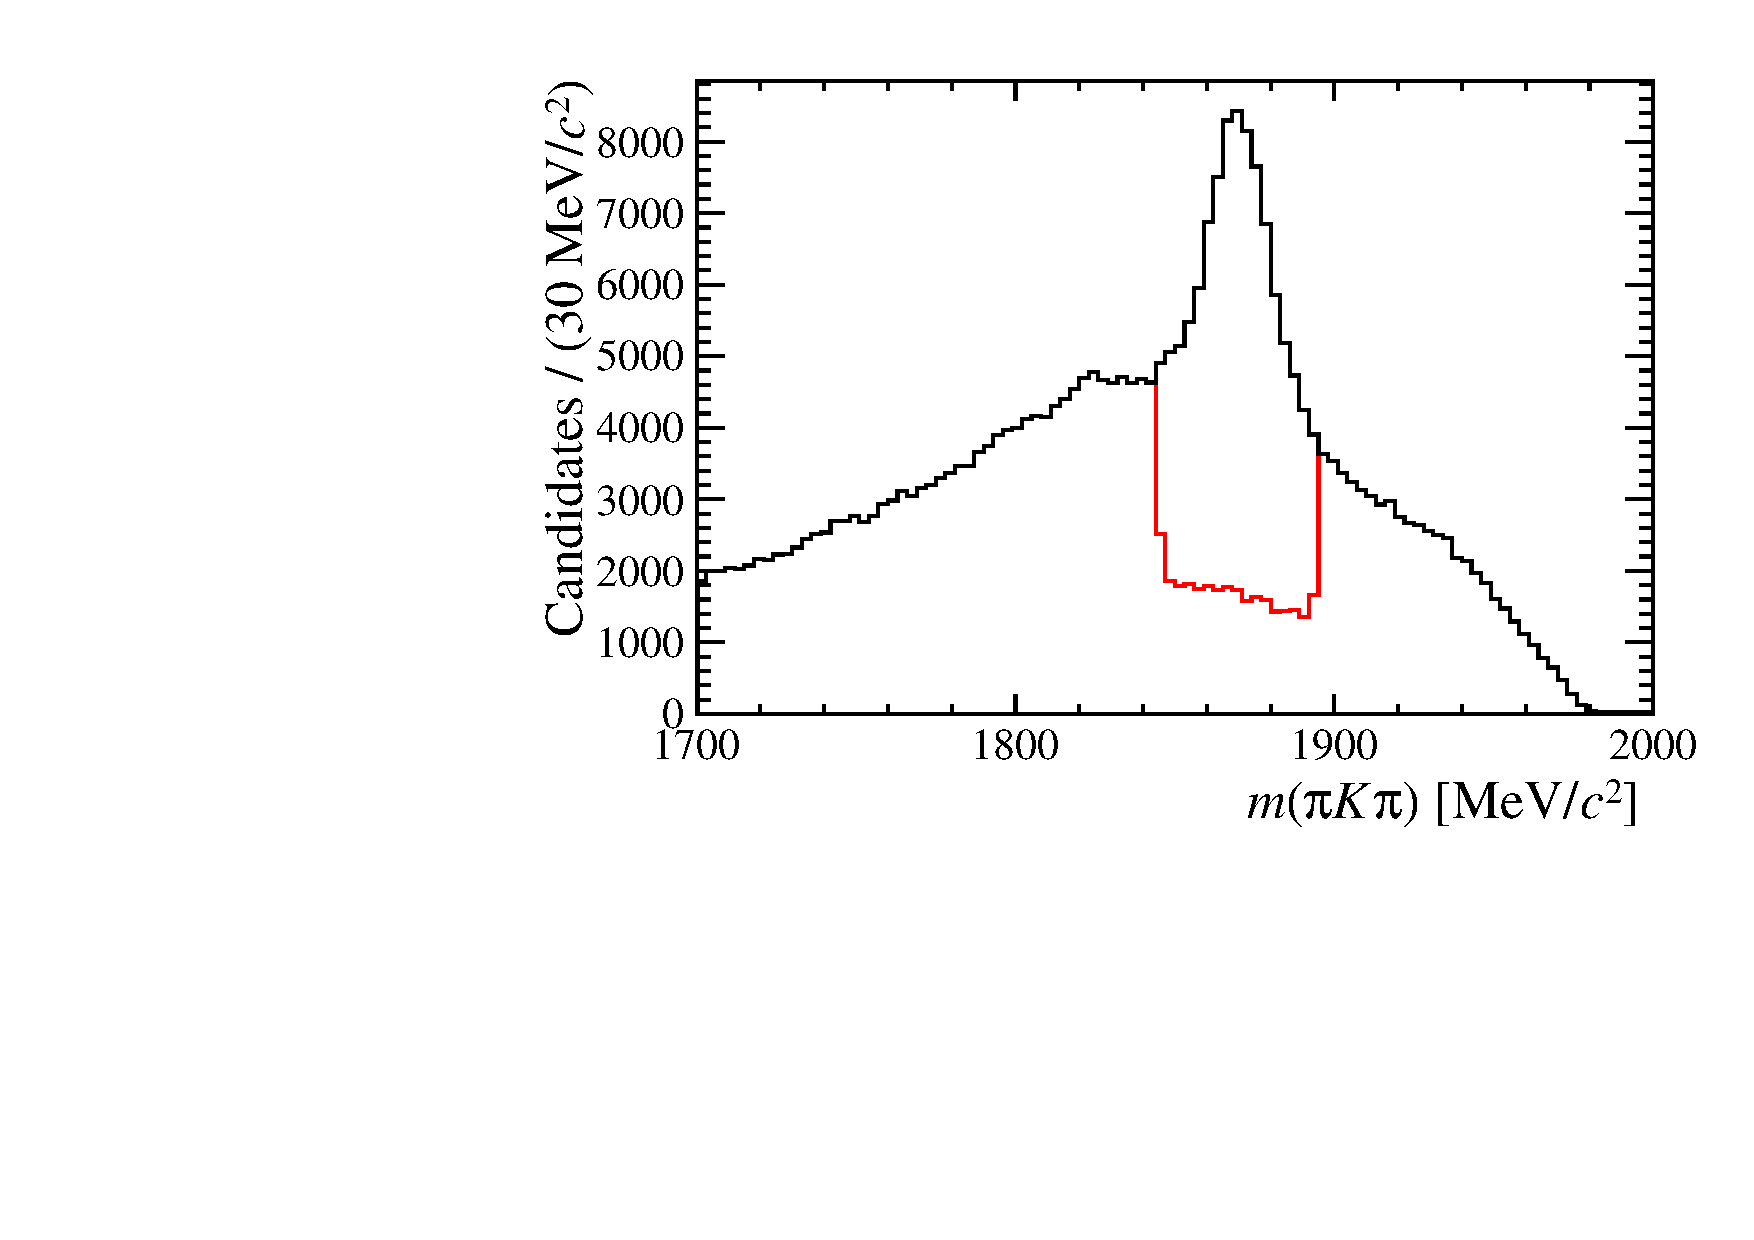
\includegraphics[width=1.0\textwidth]{figs/Selection/B2DsPhi_Ds2KKPi_D_Veto_NoBDT.pdf}
        \caption{Signal without selection}
    \end{subfigure}\\
    \begin{subfigure}[t]{0.4\textwidth}
        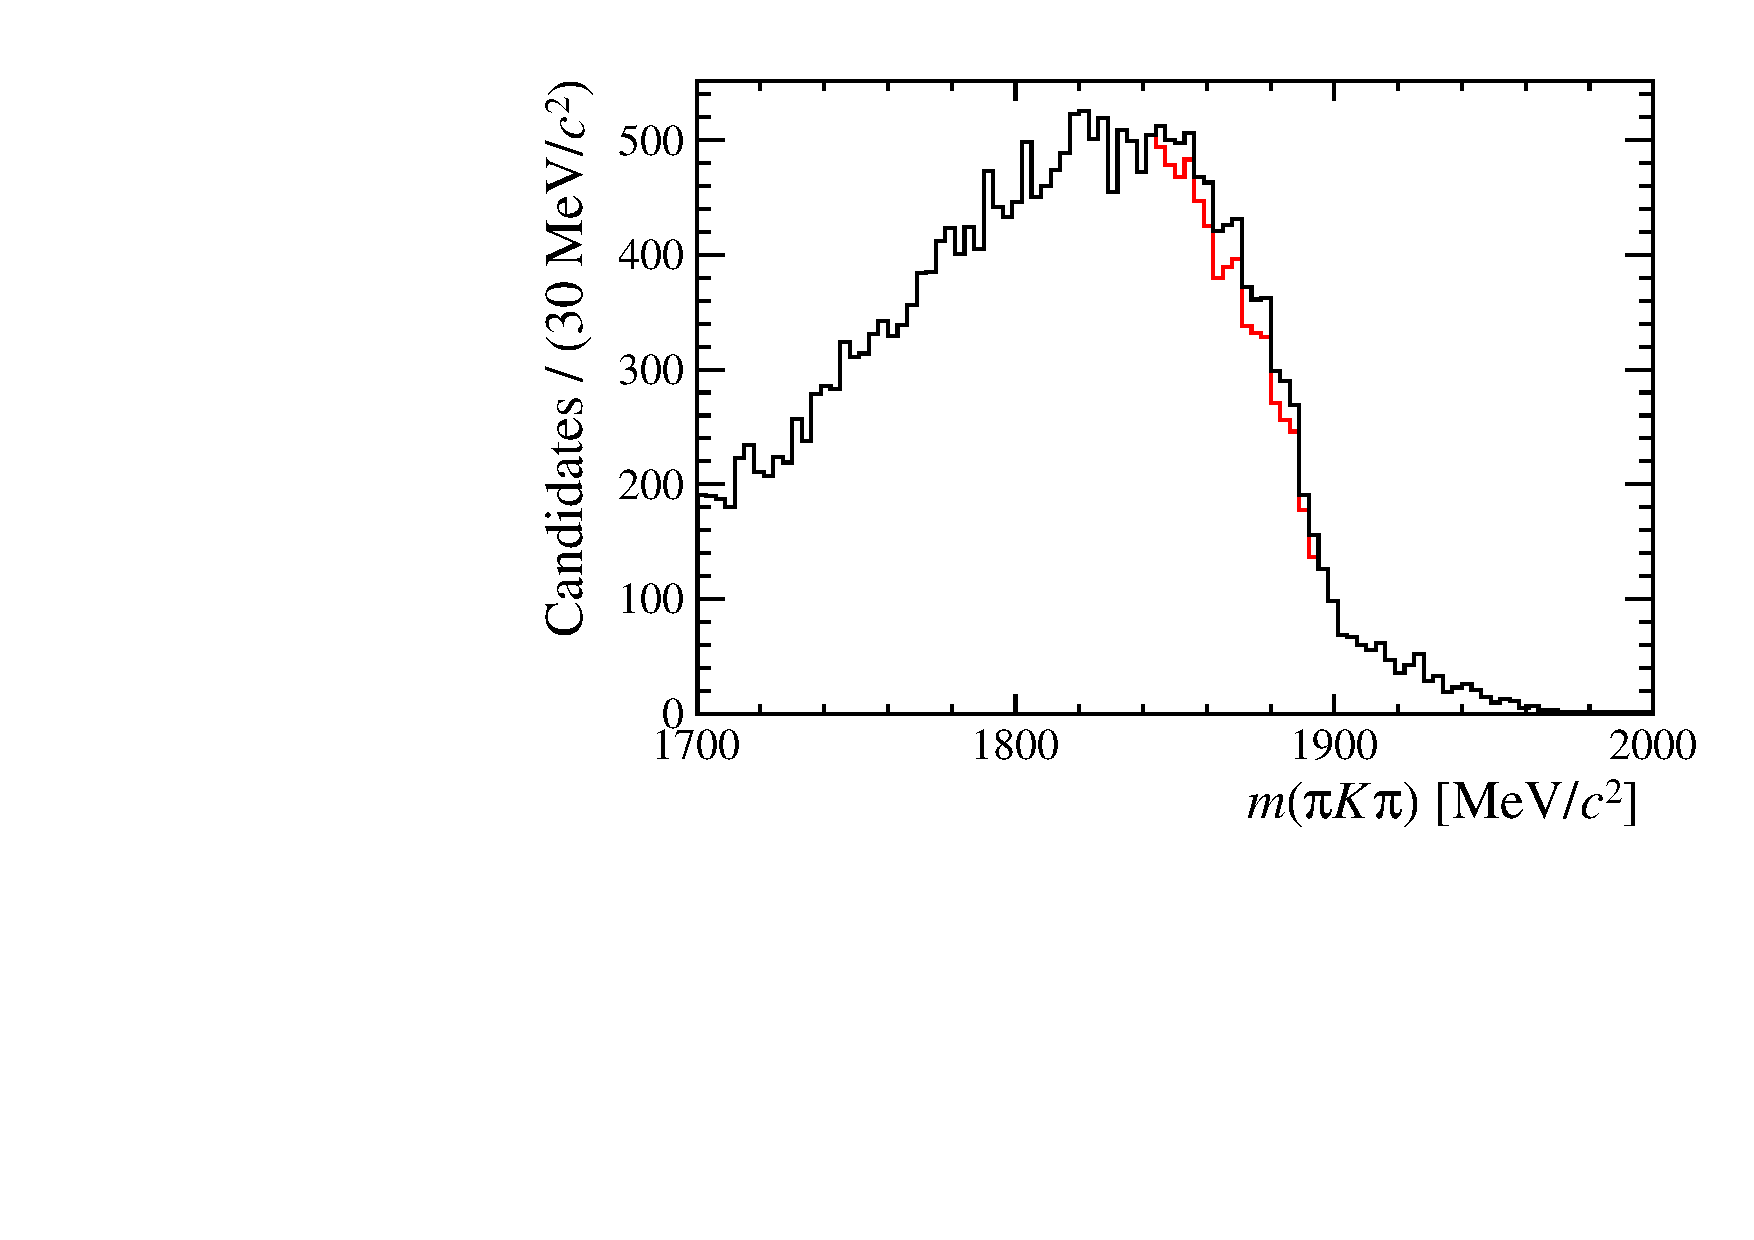
\includegraphics[width=1.0\textwidth]{figs/Selection/B2DsD0_Ds2KKPi_D_Veto_WithBDT.pdf}
        \caption{Normalisation with selection}
    \end{subfigure}%
    \begin{subfigure}[t]{0.4\textwidth}
        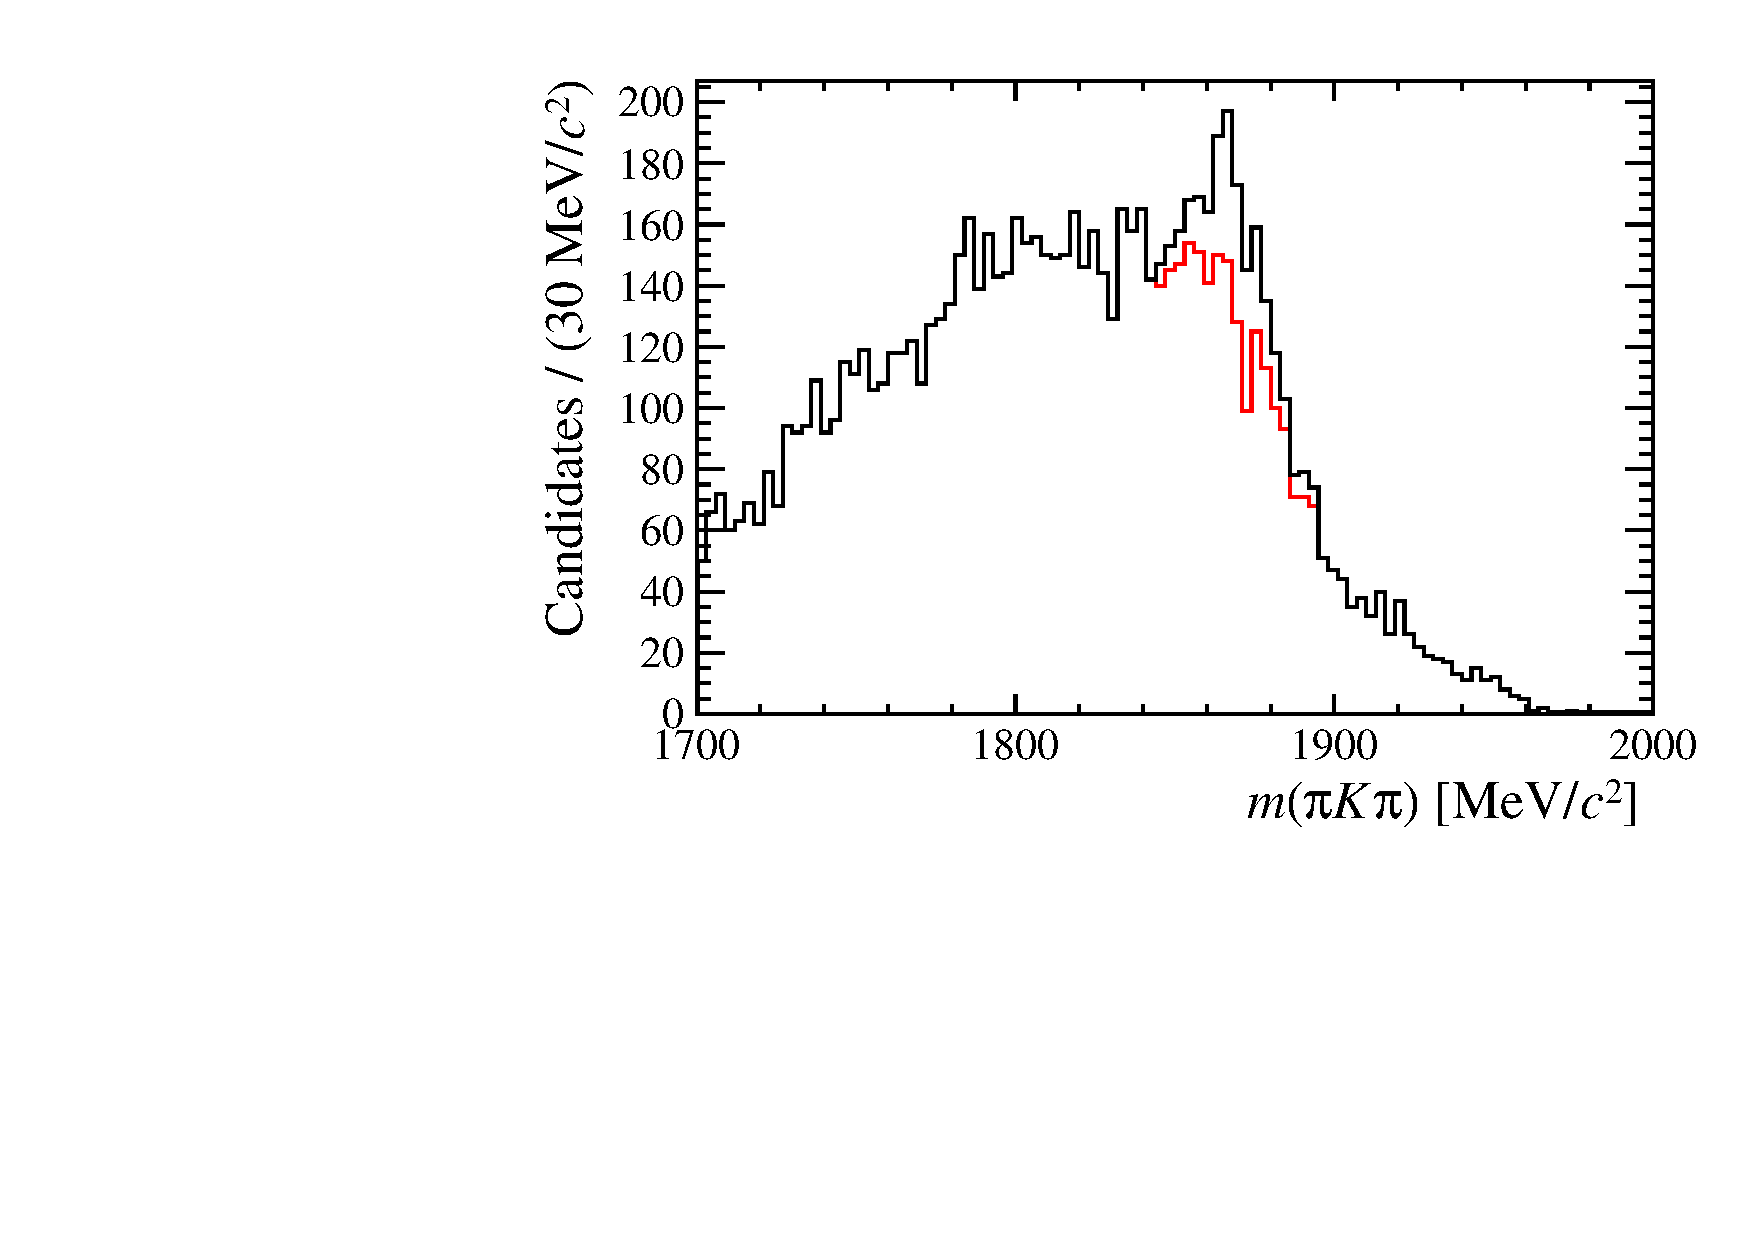
\includegraphics[width=1.0\textwidth]{figs/Selection/B2DsPhi_Ds2KKPi_D_Veto_WithBDT.pdf}
        \caption{Signal with selection}
    \end{subfigure}\\
    \caption{Invariant mass distributions of \decay{\Dsp}{\Kp\Km\pip} samples reconstructed as \decay{\Dp}{\pip\Km\pip} for the signal and normalisation samples. The samples are shown with (red) and without (black) the veto described in Sec.~\ref{sec:pidvetos}. The distributions are shown before (top) and after (bottom) the MVA requirements have been applied.}
    \label{fig:PIDVetos_Ds2KKPi_D_Veto}   
\end{figure}
%%%%%%%%%%%%%%%%%%%%%%%%%%%%%%%%%%%%%%%%%%%%%%%%%%%%%%%%%%

%%%%%%%%%%%%%%%%%%%%%%%%%%%%%%%%%%%%%%%%%%%%%%%%%%%%%%%%%%
\begin{figure}[!h]
    \centering
    \begin{subfigure}[t]{0.4\textwidth}
        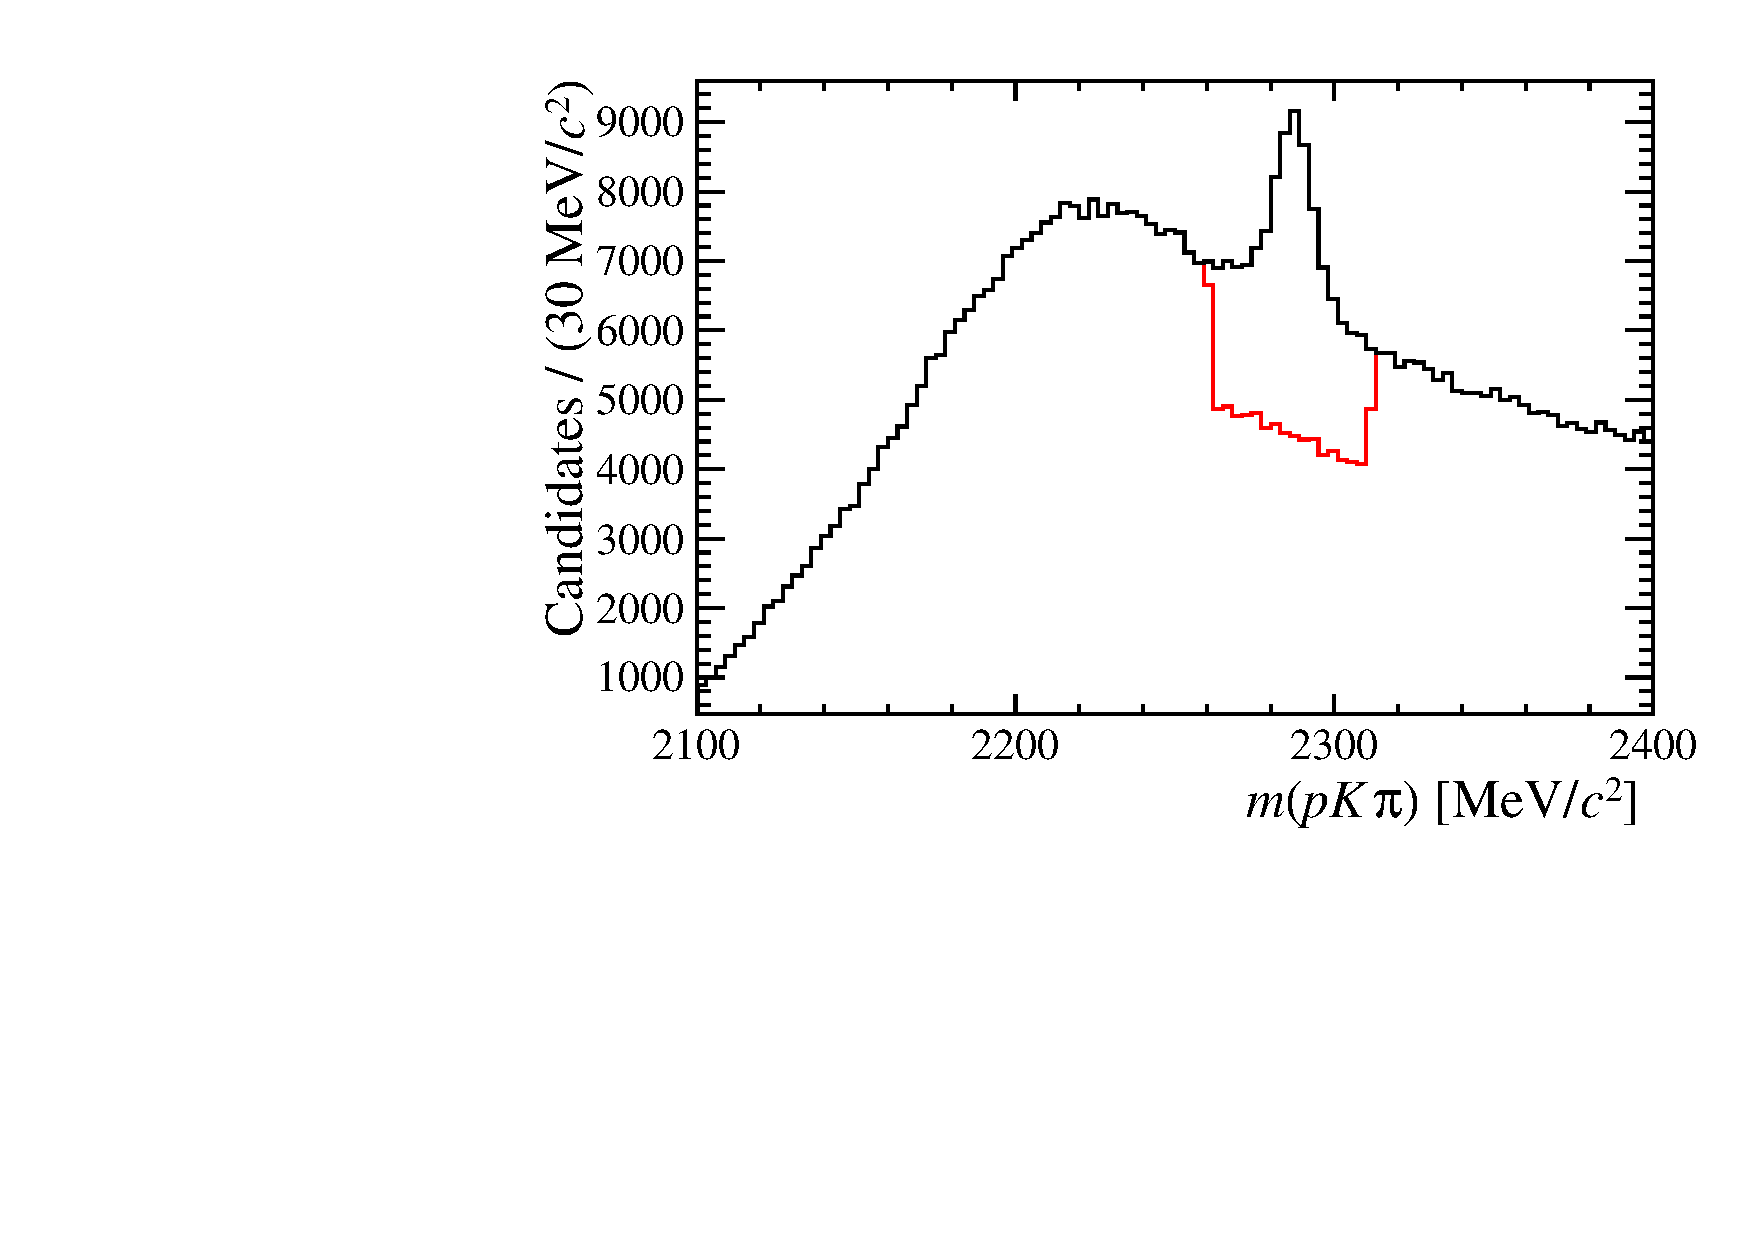
\includegraphics[width=1.0\textwidth]{figs/Selection/B2DsD0_Ds2KKPi_Lc_Veto_NoBDT.pdf}
        \caption{Normalisation without MVA cut}
    \end{subfigure}%
    \begin{subfigure}[t]{0.4\textwidth}
        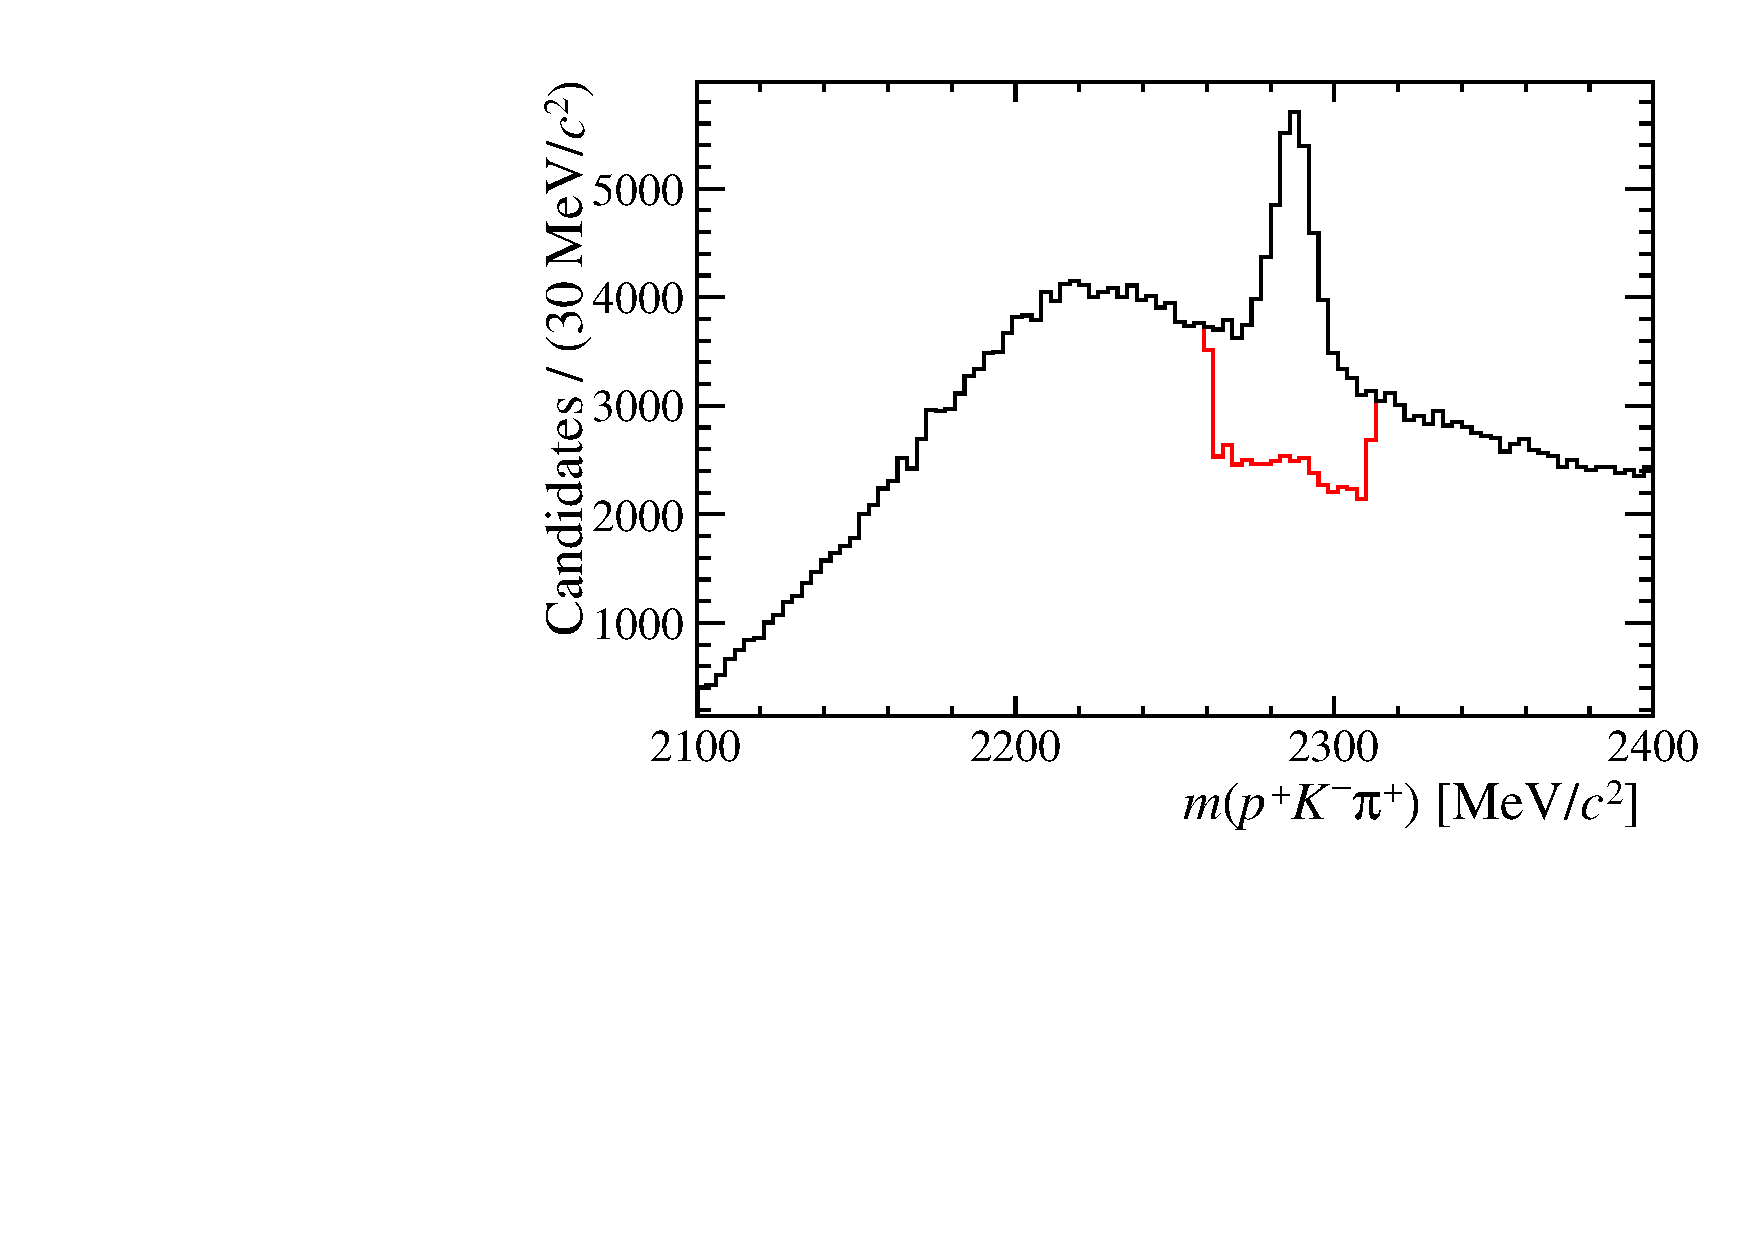
\includegraphics[width=1.0\textwidth]{figs/Selection/B2DsPhi_Ds2KKPi_Lc_Veto_NoBDT.pdf}
        \caption{Signal without MVA cut}
    \end{subfigure}\\
    \begin{subfigure}[t]{0.4\textwidth}
        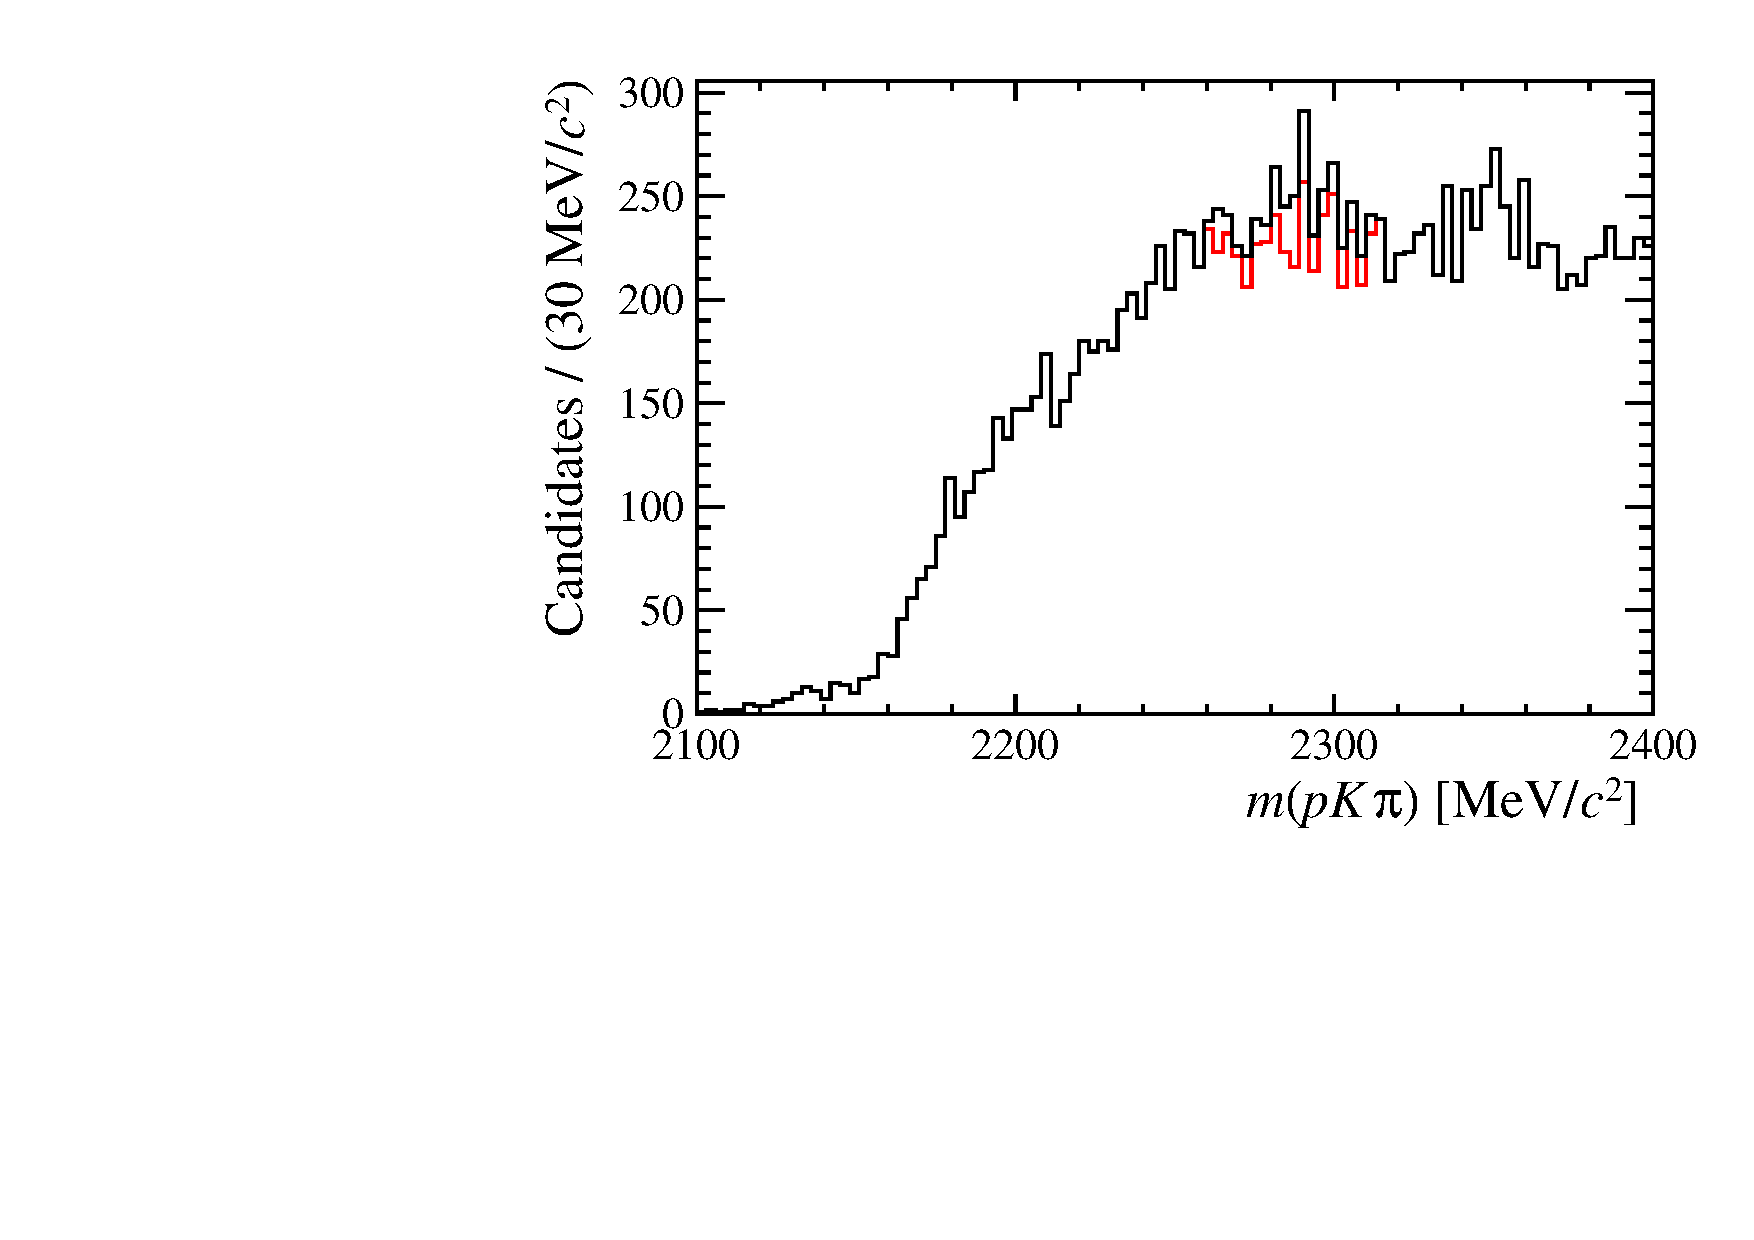
\includegraphics[width=1.0\textwidth]{figs/Selection/B2DsD0_Ds2KKPi_Lc_Veto_WithBDT.pdf}
        \caption{Normalisation with MVA cut}
    \end{subfigure}%
    \begin{subfigure}[t]{0.4\textwidth}
        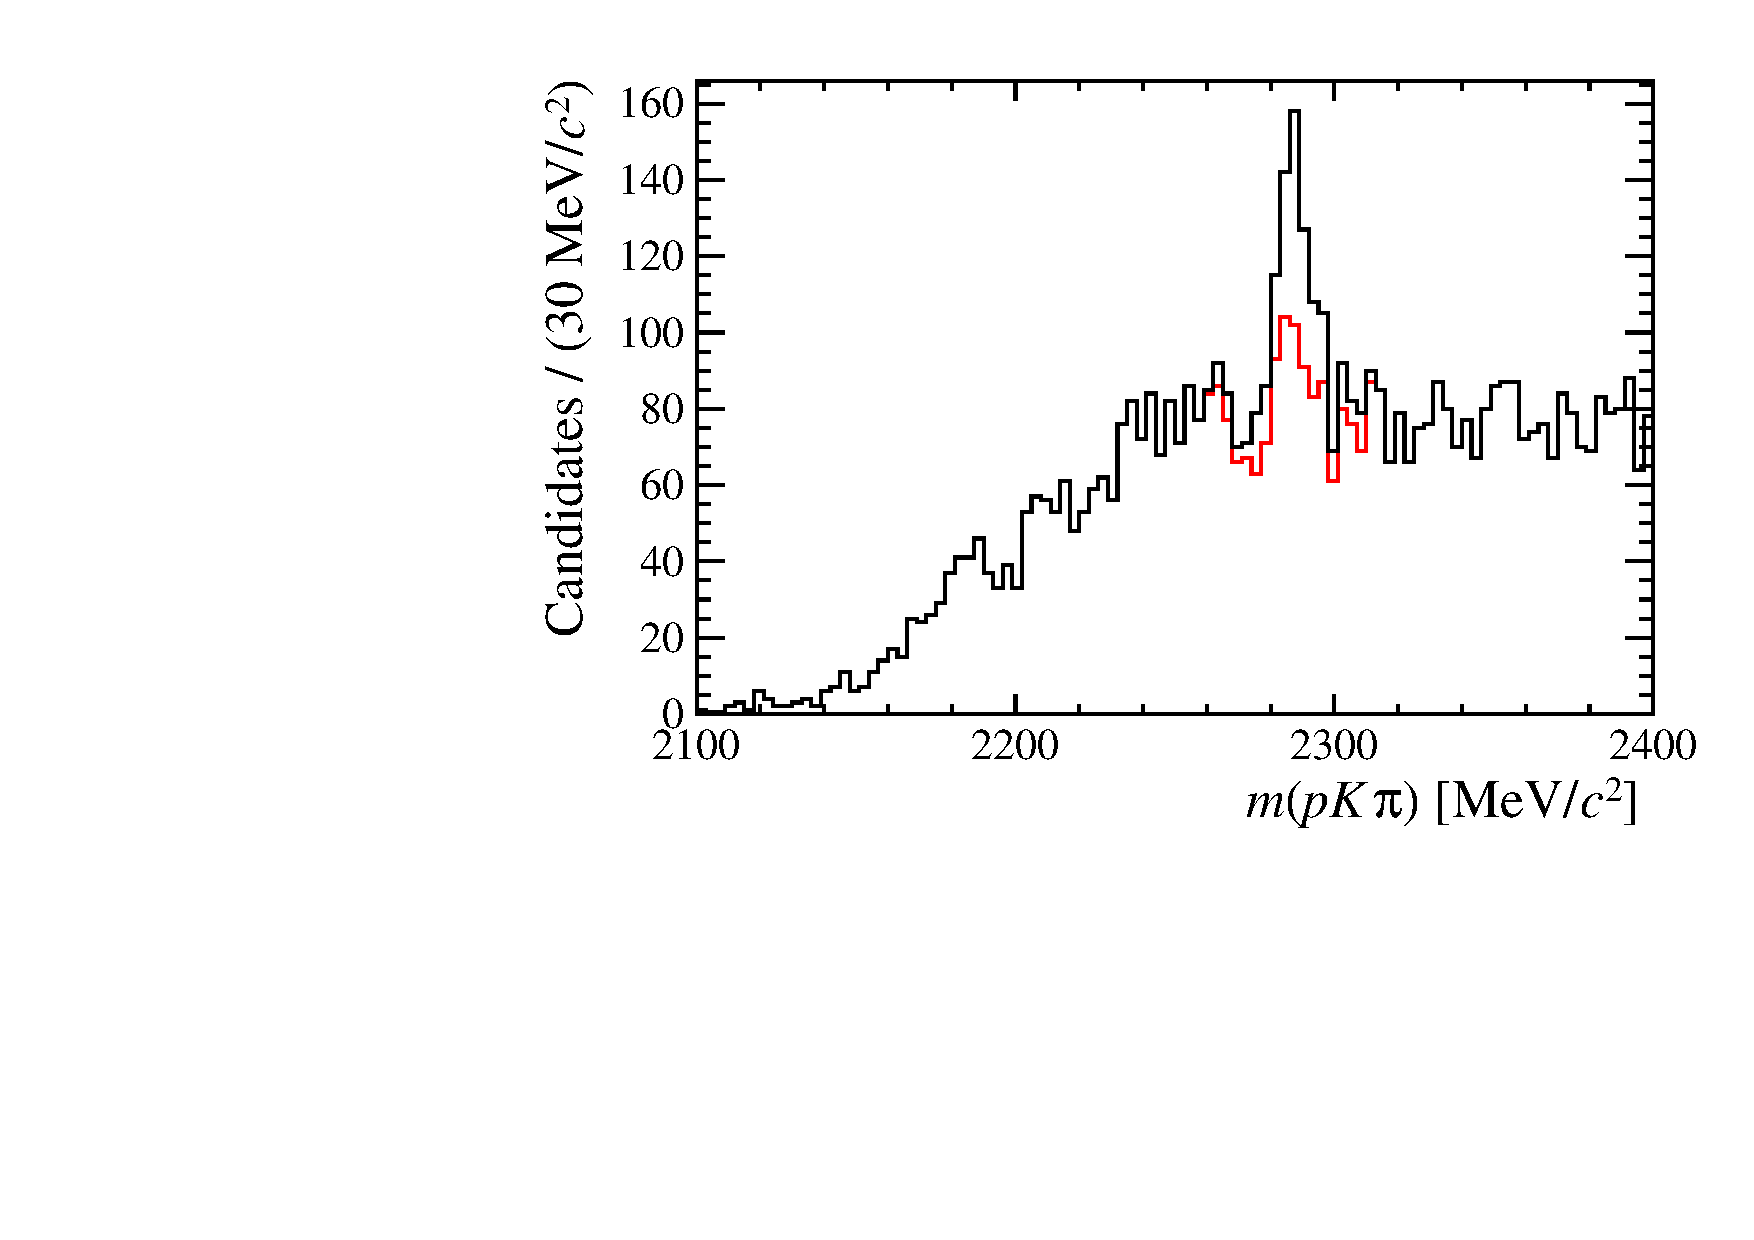
\includegraphics[width=1.0\textwidth]{figs/Selection/B2DsPhi_Ds2KKPi_Lc_Veto_WithBDT.pdf}
        \caption{Signal with MVA cut}
    \end{subfigure}\\
    \caption{Invariant mass distributions of \decay{\Dsp}{\Kp\Km\pip} samples reconstructed as \decay{\Lc}{\Pp\Km\pip} for the signal and normalisation samples. The samples are shown with (red) and without (black) the veto described in Sec.~\ref{sec:pidvetos}. The distributions are shown before (top) and after (bottom) the MVA requirements have been applied.}
    \label{fig:PIDVetos_Ds2KKPi_Lc_Veto}   
\end{figure}
%%%%%%%%%%%%%%%%%%%%%%%%%%%%%%%%%%%%%%%%%%%%%%%%%%%%%%%%%%

{\color{Red}
\begin{itemize}
\item Include Descriptions
\item Include plots of each applied
\end{itemize}
}

\subsection{Invariant mass vetoes}
\label{sec:kinematicvetos}

Sharp peaking structures are observed in subsets of the final state particles. These are removed with simple invariant mass cuts to remove combinatorial or partially reconstructed backgrounds that result from these incorrectly reconstructed decays. 
For simplicity the final state particles for each mode are labelled with a number between 1--5 as described in Table~\ref{table:vetolabels}.

\begin{table*}[!ht]
\begin{center}
\begin{tabular}{ l c c c c c c }
\hline
Decay Mode & 1  & 2 & 3 & 4 & 5 \\
\hline
\decay{\Bp}{(\decay{\Dsp}{\Kp\Km\pip})\phiz}       & \Kp    & \Km    & \pip  & \Kp  & \Km \\
\decay{\Bp}{(\decay{\Dsp}{\pip\pim\pip})\phiz}     & \pip   & \pim   & \pip  & \Kp  & \Km \\
\decay{\Bp}{(\decay{\Dsp}{\Kp\pim\pip})\phiz}      & \Kp    & \pim   & \pip  & \Kp  & \Km \\
\hline
\decay{\Bp}{(\decay{\Dsp}{\Kp\Km\pip})\Kp\Km}      & \Kp    & \Km    & \pip  & \Kp  & \Km \\
\hline
\end{tabular}
\caption{Particle labels used when studying invariant mass vetoes for \decay{\Bp}{\Dsp\phiz} and \decay{\Bp}{\Dsp\Kp\Km} candidates.}
\label{table:vetolabels}
\end{center}
\end{table*}

All combinations of the final state particles that create a neutral or singly-charged candidate are investigated.
Significant structures are observed for all three \Dsp decay modes in some combination. 

The following vetos are applied to remove these incorrectly reconstructed decays.
\begin{itemize}
\item For the mode \decay{\Bp}{(\decay{\Dsp}{\Kp\Km\pip})\phiz}
\begin{itemize}
\item $|m(\text{1245})- m(\Bs)| > 50\mevcc$
\item $|m(\text{345})- m(\Dsp)| > 25\mevcc$ and $|m(\text{345})- m(\Dp)| > 25\mevcc$
\end{itemize}

\item For the mode \decay{\Bp}{(\decay{\Dsp}{\pip\pim\pip})\phiz}
\begin{itemize}
\item $|m(\text{145})- m(\Dsp)| > 25\mevcc$ and $|m(\text{145})- m(\Dp)| > 25\mevcc$
\item $|m(\text{245})- m(\Dsp)| > 25\mevcc$ and $|m(\text{245})- m(\Dp)| > 25\mevcc$
\item $|m(\text{345})- m(\Dsp)| > 25\mevcc$ and $|m(\text{345})- m(\Dp)| > 25\mevcc$
\end{itemize}
\item For the mode \decay{\Bp}{(\decay{\Dsp}{\Kp\pim\pip})\phiz}
\begin{itemize}
\item $|m(\text{245})- m(\Dsp)| > 25\mevcc$ and $|m(\text{245})- m(\Dp)| > 25\mevcc$
\item $|m(\text{345})- m(\Dsp)| > 25\mevcc$ and $|m(\text{345})- m(\Dp)| > 25\mevcc$
\end{itemize}
{\color{Red}
\item For the mode \decay{\Bp}{(\decay{\Dsp}{\Kp\Km\pip})\Kp\Km}
\begin{itemize}
\item $|m(\text{1245})- m(\Bs)| > 50\mevcc$
\item $|m(\text{345})- m(\Dsp)| > 25\mevcc$ and $|m(\text{345})- m(\Dp)| > 25\mevcc$
\end{itemize}
}
\end{itemize}


%%%%%%%%%%%%%%%%%%%%%%%%%%%%%%%%%%%%%%%%%%%%%%%%%%%%%%%%%%
\begin{figure}[!h]
   \centering
   \begin{subfigure}[t]{1.0\textwidth}
      \centering
      \begin{subfigure}[t]{0.32\textwidth}
         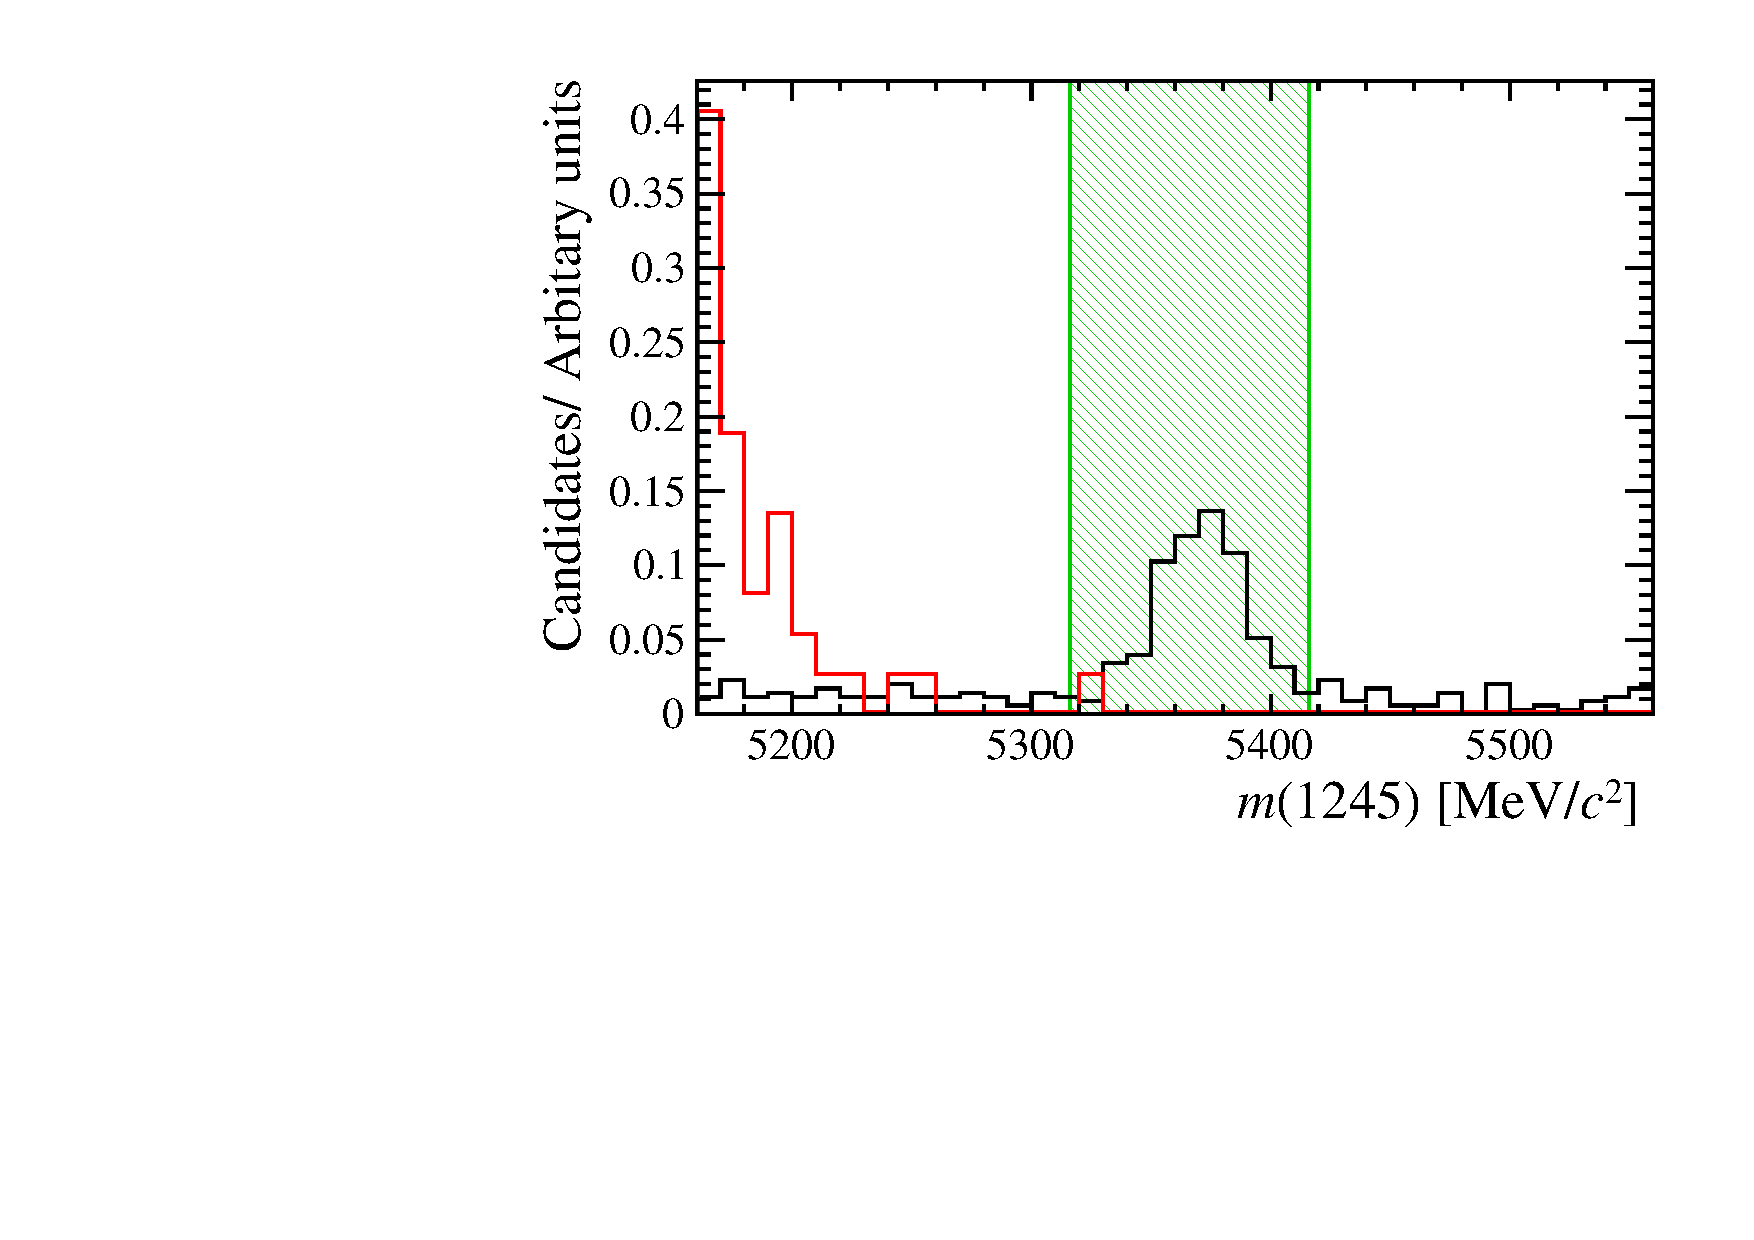
\includegraphics[width=1.0\textwidth]{figs/Selection/Veto_Comparison_B2DsPhi_Ds2KKPi_m1245.pdf}
      \end{subfigure}
      \begin{subfigure}[t]{0.32\textwidth}
         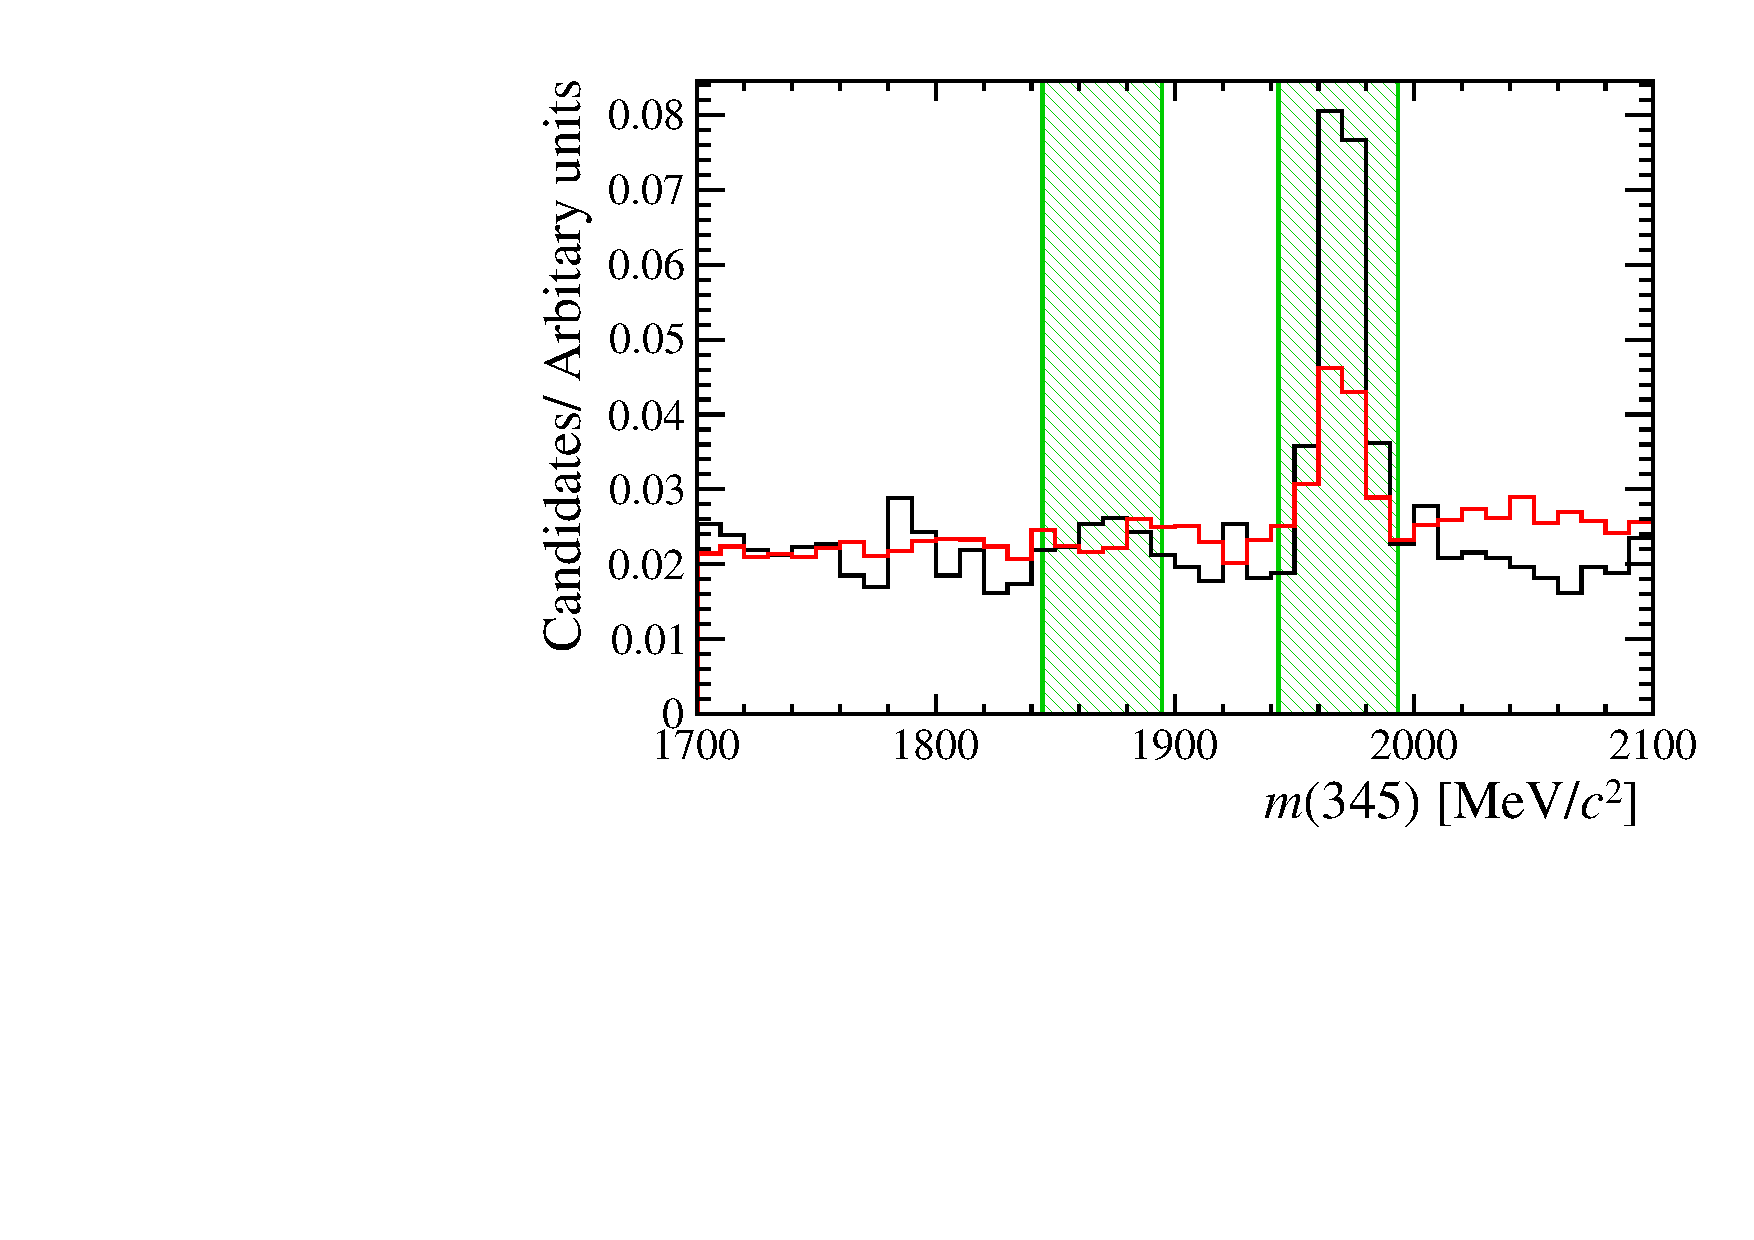
\includegraphics[width=1.0\textwidth]{figs/Selection/Veto_Comparison_B2DsPhi_Ds2KKPi_m345.pdf}
      \end{subfigure}
      \caption{\decay{\Bp}{(\decay{\Dsp}{\Kp\Km\pip})\phiz}}
   \end{subfigure}
   \begin{subfigure}[t]{1.0\textwidth}
      \centering
      \begin{subfigure}[t]{0.32\textwidth}
         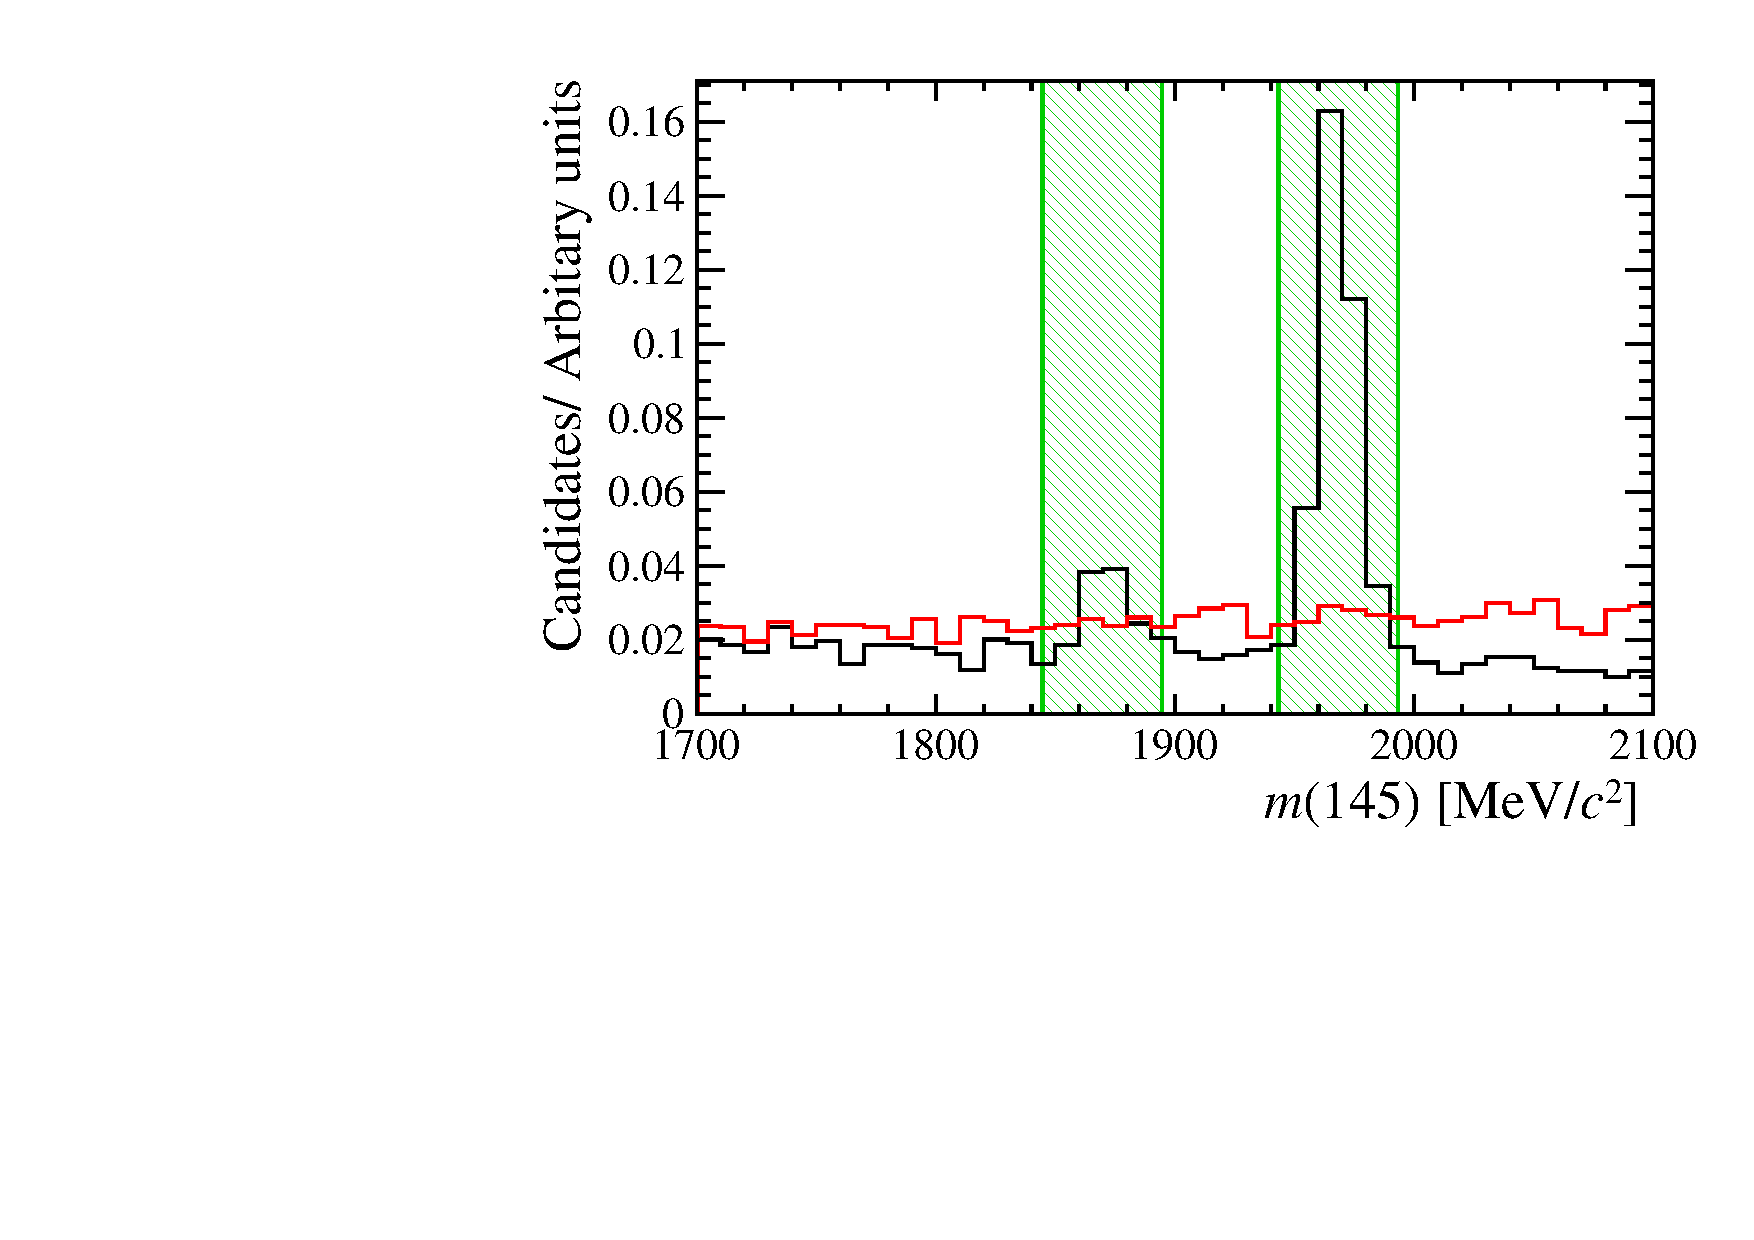
\includegraphics[width=1.0\textwidth]{figs/Selection/Veto_Comparison_B2DsPhi_Ds2PiPiPi_m145.pdf}
      \end{subfigure}
      \begin{subfigure}[t]{0.32\textwidth}
         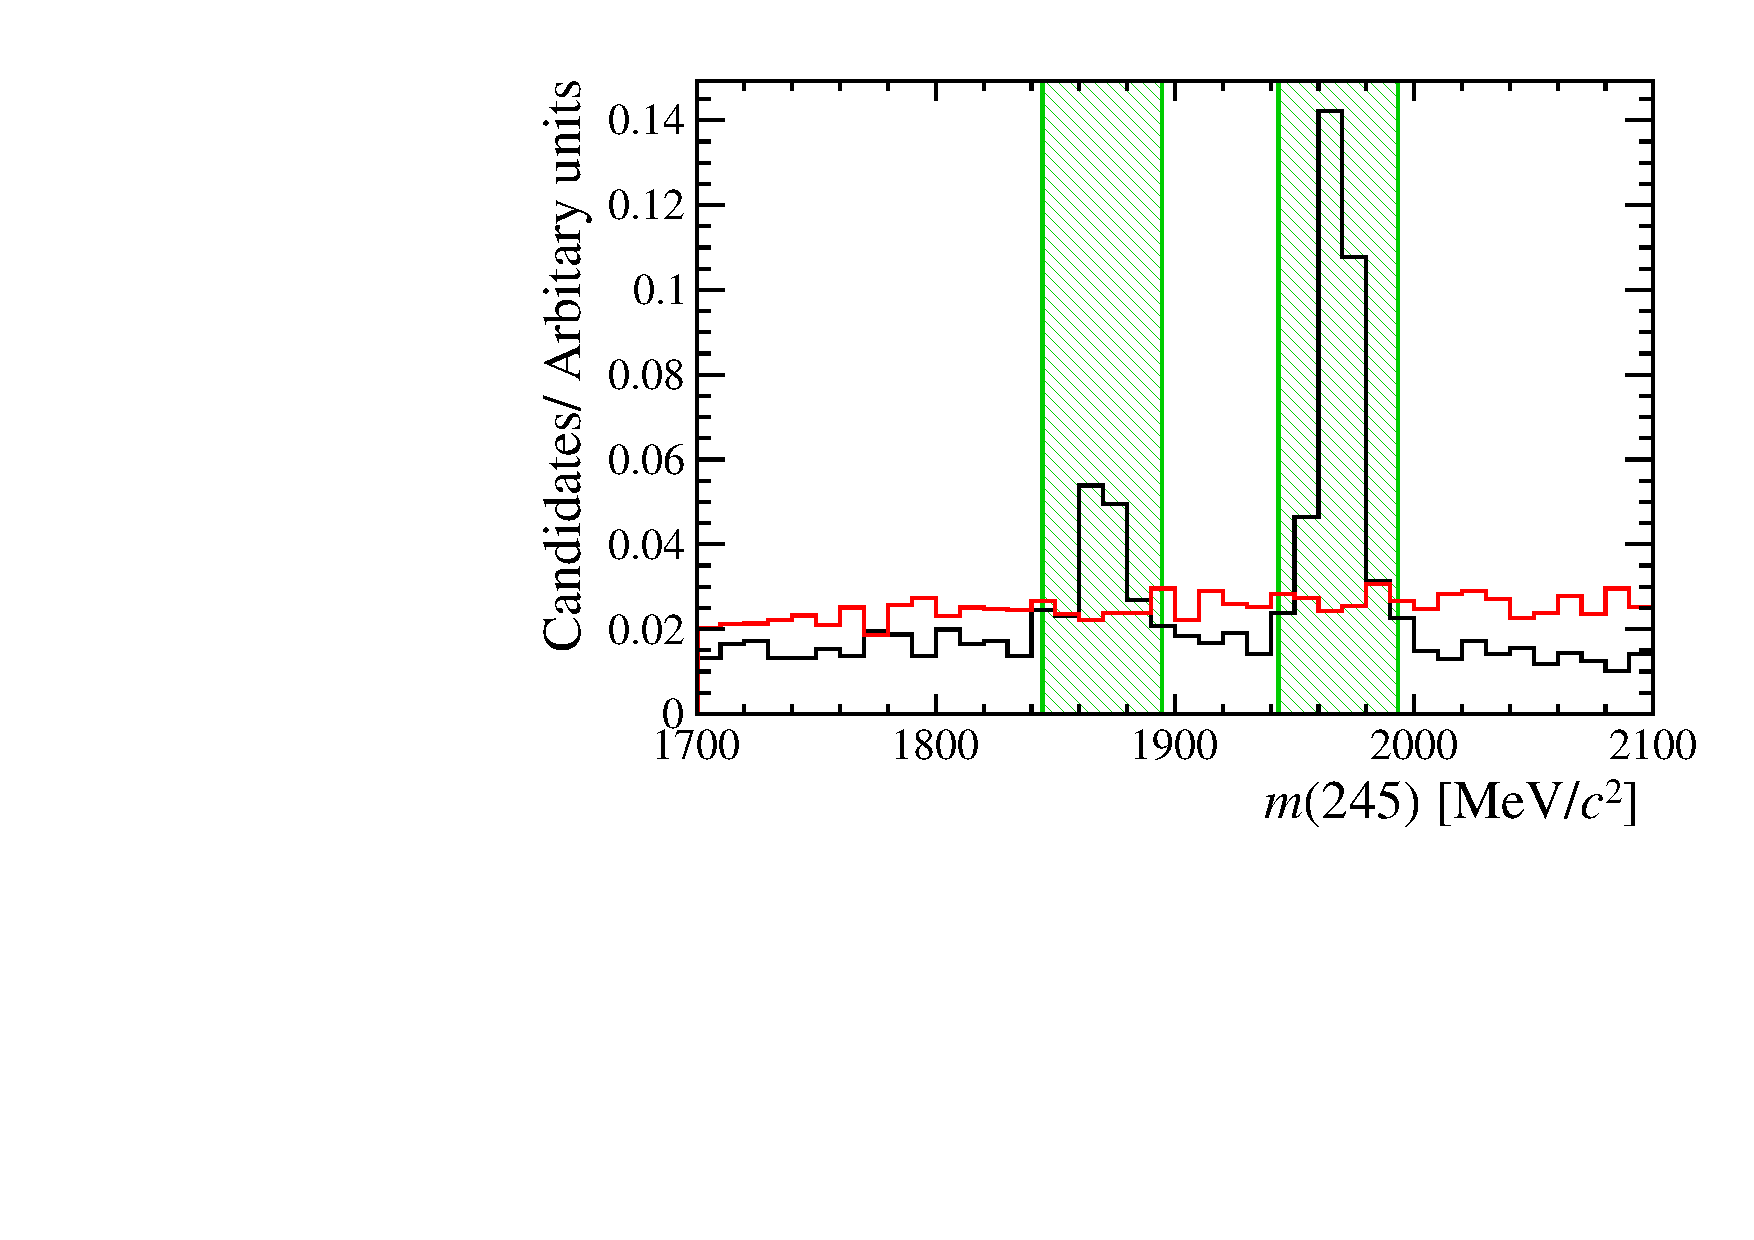
\includegraphics[width=1.0\textwidth]{figs/Selection/Veto_Comparison_B2DsPhi_Ds2PiPiPi_m245.pdf}
      \end{subfigure}
      \begin{subfigure}[t]{0.32\textwidth}
         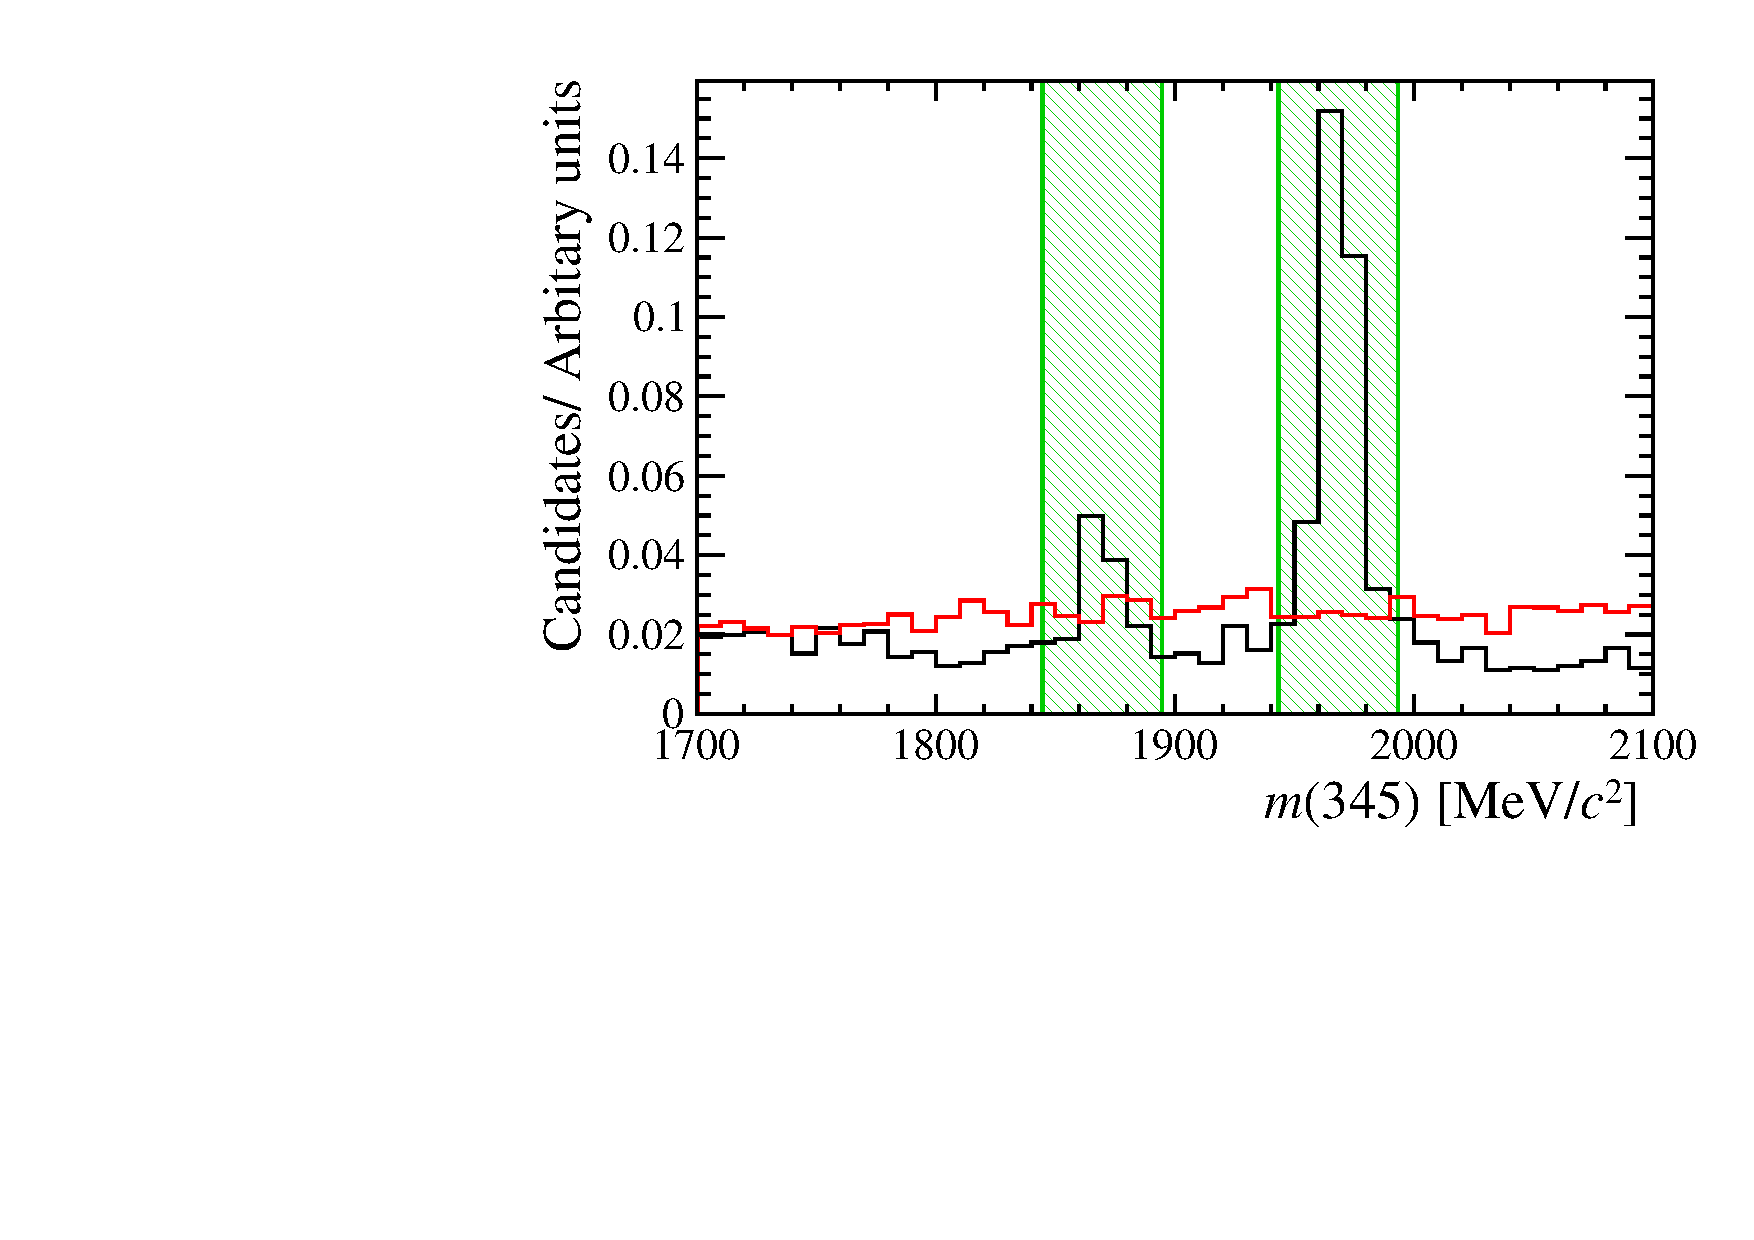
\includegraphics[width=1.0\textwidth]{figs/Selection/Veto_Comparison_B2DsPhi_Ds2PiPiPi_m345.pdf}
      \end{subfigure}
      \caption{\decay{\Bp}{(\decay{\Dsp}{\pip\pim\pip})\phiz}}
   \end{subfigure}
   \begin{subfigure}[t]{1.0\textwidth}
      \centering
      \begin{subfigure}[t]{0.32\textwidth}
         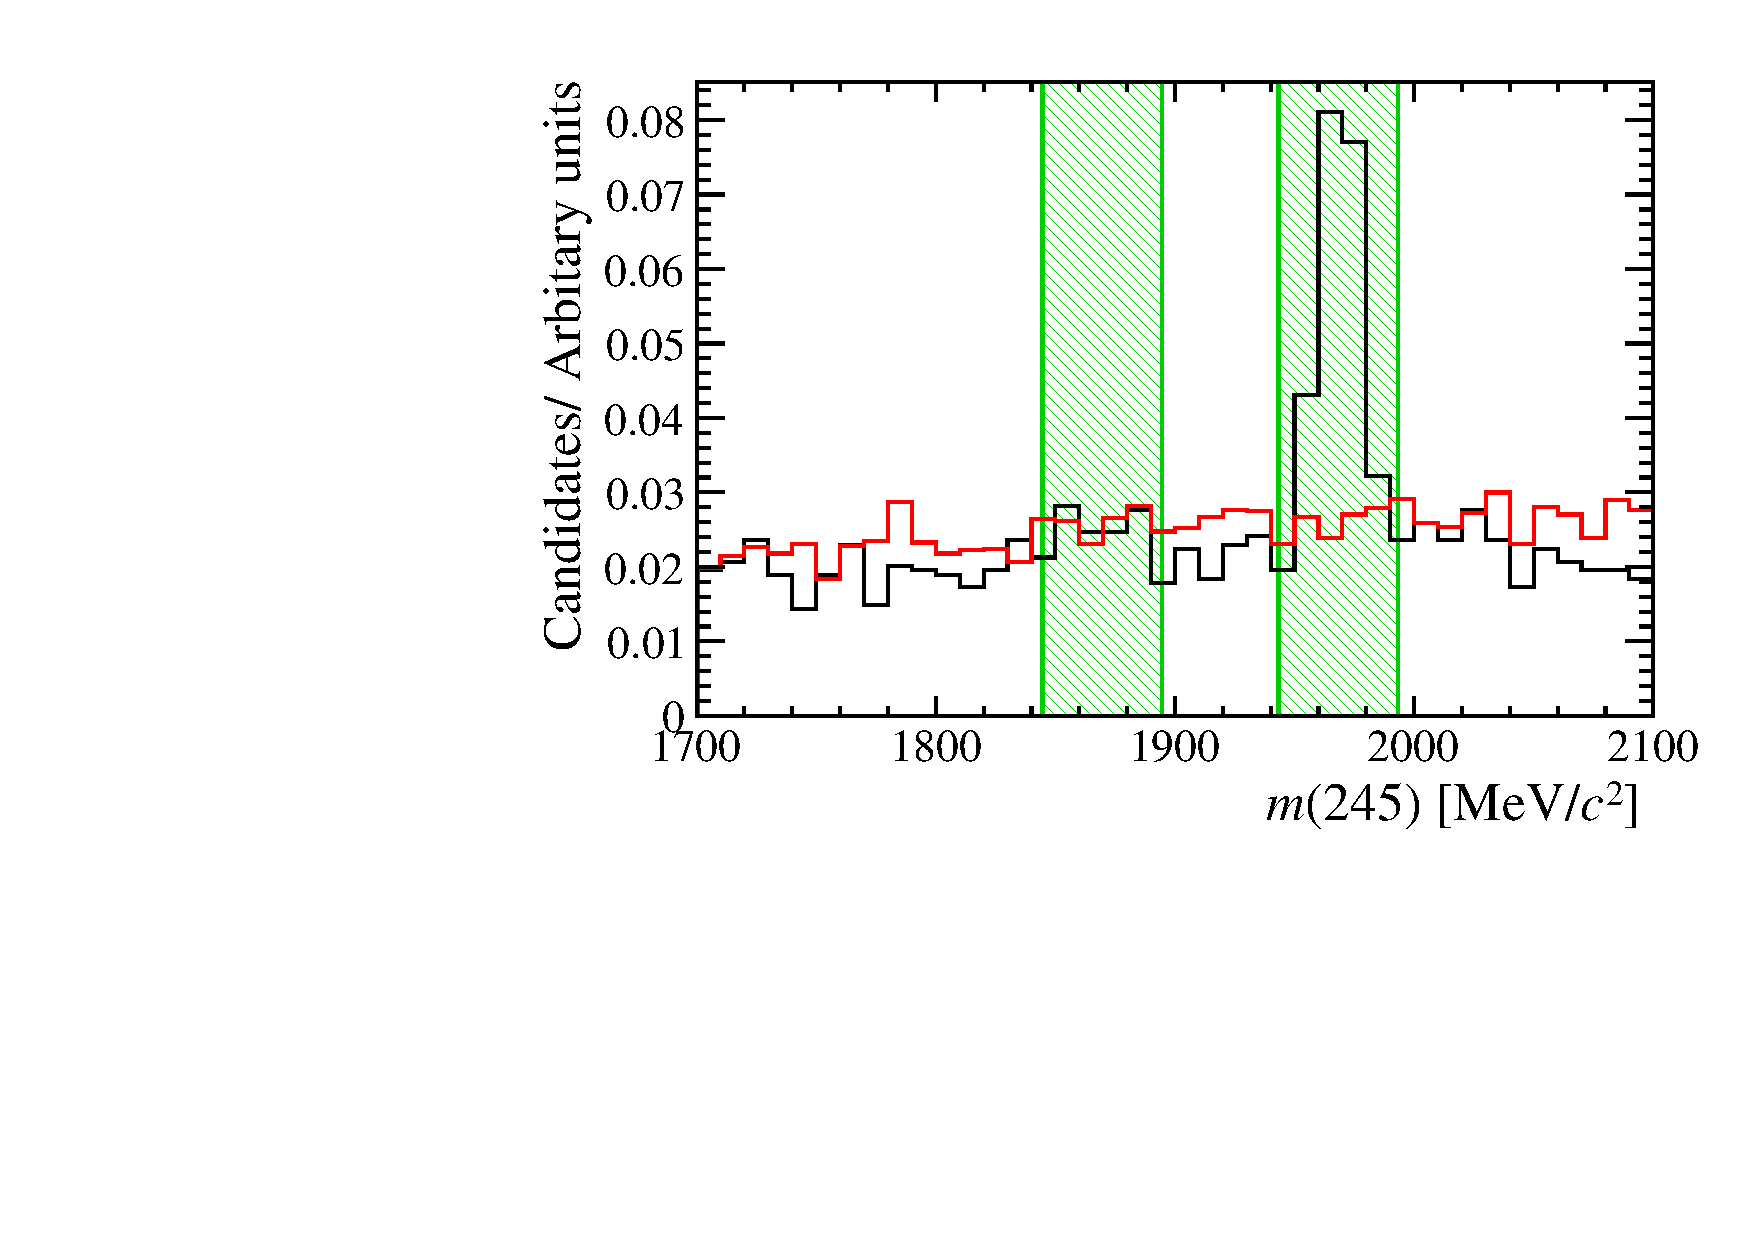
\includegraphics[width=1.0\textwidth]{figs/Selection/Veto_Comparison_B2DsPhi_Ds2KPiPi_m245.pdf}
      \end{subfigure}
      \begin{subfigure}[t]{0.32\textwidth}
         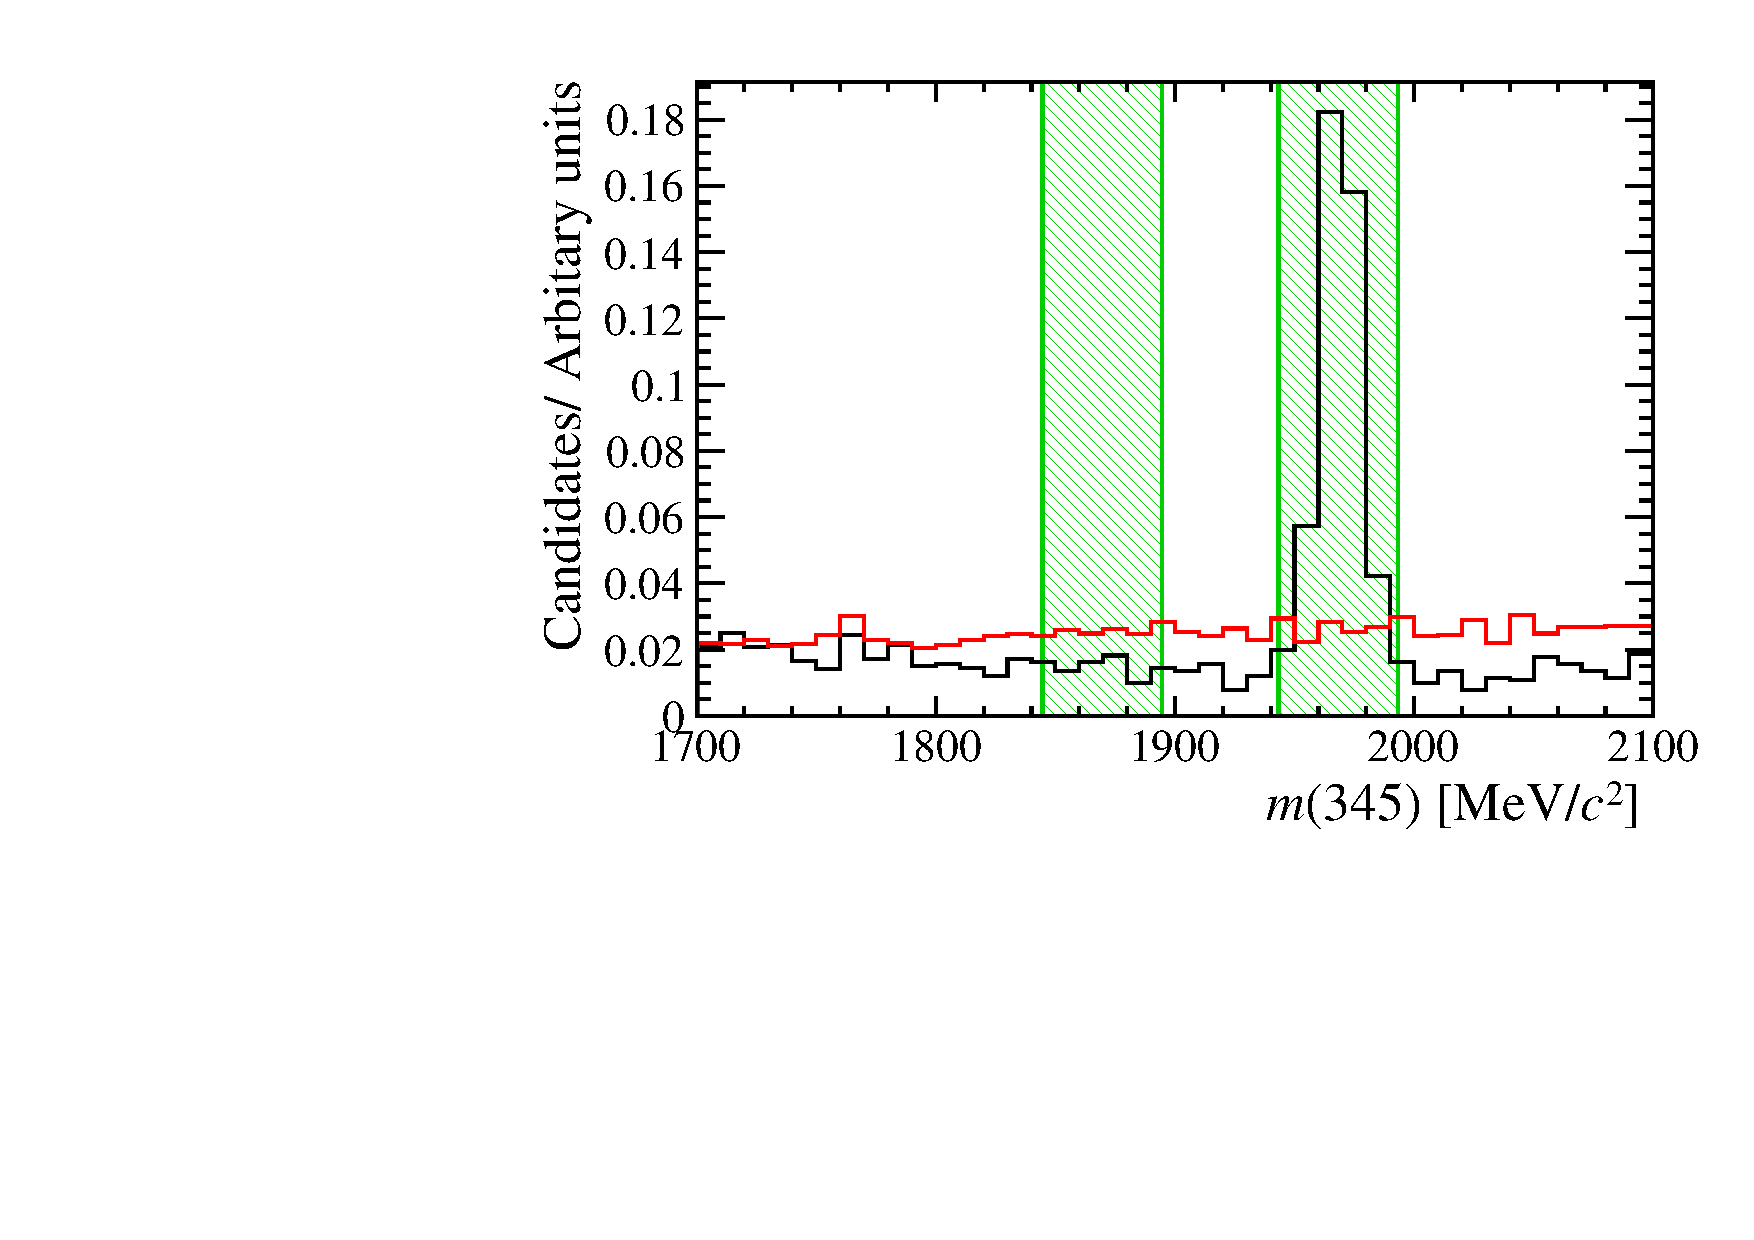
\includegraphics[width=1.0\textwidth]{figs/Selection/Veto_Comparison_B2DsPhi_Ds2KPiPi_m345.pdf}
      \end{subfigure}
      \caption{\decay{\Bp}{(\decay{\Dsp}{\Kp\pim\pip})\phiz}}
   \end{subfigure}

   \caption{Invariant mass distributions for subsets of decay products. The green region show the regions removed by the vetoes listed in Sec~\ref{sec:kinematicvetos}.}
   \label{fig:invariantmassvetoes}   
\end{figure}
%%%%%%%%%%%%%%%%%%%%%%%%%%%%%%%%%%%%%%%%%%%%%%%%%%%%%%%%%%



In the search for \decay{\Bp}{\Dsp\Kp\Km} decays the increased size of the $m(\Kp\Km)$ phase space means more 



\subsection{Normalisation mode veto}
\label{sec:normvetos}

In the search for \decay{\Bp}{\Dsp\Kp\Km} decays, the phase space 

\subsection{Multivariate analysis}

Multivariate Analyses (MVAs) are used to help discriminate between genuine \Dsp and \phiz meson decays and combinations of unrelated particles. 
These MVAs are trained using large samples of candidates from other \B mesons decays in data with similar topologies. 
This data-driven approach can benefit from an expanded set of variables that are not perfectly represented in simulation, including track quality and particle identification information, in addition to the kinematic and geometric properties.
The sample of \Dsp mesons is obtained from the relatively abundant \decay{\Bsb}{\Dsp\pim} decay. Similarly, the sample of \phiz mesons is obtained from \decay{\Bs}{\jpsi\phiz} decays. Large, high purity samples are reconstructed using similar requirements to those applied in the selection of signal \Dsp and \phiz mesons.
A sample is selected for each of the \Dsp and \phiz meson decays uses in this analysis, as listed in Table~\ref{tab:mva_modes}. 
These samples are used to select each of the 

\begin{table}[t]
 \caption{MVA modes}
\begin{center}\begin{tabular}{lll}
   \hline
   Sample                    & Mode                       & Use \\ 
   \hline
   \decay{\Bsb}{\Dsp\pim}    & \decay{\Dsp}{\Kp\Km\pip}   & Training, Efficiency \\
   \decay{\Bsb}{\Dsp\pim}    & \decay{\Dsp}{\Kp\pim\pip}  & Training, Efficiency \\
   \decay{\Bsb}{\Dsp\pim}    & \decay{\Dsp}{\pip\pim\pip} & Training, Efficiency \\
   \decay{\Bs}{\jpsi\phiz}   & \decay{\phiz}{\Kp\Km}      & Training, Efficiency \\
   \hline
   \decay{\Bp}{\Dzb\pip}     & \decay{\Dzb}{\Kp\Km}       & Efficiency          \\
   \hline
 \end{tabular}\end{center}
\label{tab:mva_modes}
\end{table}


%% Describe fits, sWeights and signal/background samples
The train variable distributions for the \Dsp and \phiz meson samples are isolated by background subtracting the \decay{\Bs}{\jpsi\phiz} and \decay{\Bsb}{\Dsp\pim} decays using the \sPlot technique~\cite{Pivk:2004ty}. Unbinned maximum likelihood fits are performed to the \Dsp and \phiz invariant mass distribution in order to determine the yield of \Dsp and \phiz candidates respectively. These fits are performed separately for each year of data taking, and for each of the targeted decays. 

{\color{Blue}
-The $\phi$ and $\Dsp$ invariant mass distributions are fitted separately for each year. 
- The training uses the \phiz or \Dsp sidebands as a background sample.
}

%% Discussion of input variables
The MVA method is trained using a large set of variables chosen to help discriminate between the signals of interest and combinations of unrelated tracks.

{\color{Blue}

-These are selected using dedicated Stripping Lines designed to select decays. To ensure these samples are representative of the target decays, a preselection is applied to the data. This comprises of similar trigger, background veto and PID requirements applied to the signal modes.
}

%% Discussion of MVA technicalities 
The MVA method chosen in this analysis is a gradient Boosted Decision Tree (BDTG)~\cite{Breiman}. This is implemented using the \emph{TMVA} package as part of the \emph{ROOT} framework. 
%% CHECK This method was compared to a BDT and bagged-BDT 


A total of eight MVAs are trained to target the decays \decay{\phi}{\Kp\Km}, \decay{\Dsp}{\Kp\Km\pip}, \decay{\Dsp}{\Kp\pim\pip} and \decay{\Dsp}{\pip\pim\pip}, separately in the Run 1 (2011 and 2012) and Run 2 (2015 and 2016) data.

The samples are split into two random but reproducible subsamples. One is used to train the corresponding MVA, the other to test its response. 

%% Optimisation 


{\color{Red}
\begin{itemize}
\item Include plots example samples
\item Include training variable distributions
\item comparision of different MVA methods
\item explicit BDTG configuration
\item Include description of what each variable means \eg ProbNN vars
\item Variable ranks
\item Discussion of overtraining and crosschecks
\item Comparison to alternative? 
\end{itemize}
}
 
%A preselection including the trigger, vetoes and PID requirements previously discussed is applied to the training samples, ensuring they are representative of the target signal decays. 


The selection criteria for each of the BDTG classifiers are determined by optimising the Punzi figure of merit~\cite{Punzi:2003bu}, 
\begin{equation}
\frac{\epsilon_{s}}{(\frac{a}{2} + \sqrt{N_{\text{BKG}}})}
\end{equation}
with $a=5$, where $\epsilon_{s}$ is the signal efficiency and $N_{\text{BKG}}$ is the number of background candidates determined from fits to data, calculated in the signal region.

{\color{Red}
\begin{itemize}
\item Include plots of optimisation
\end{itemize}
}

%% Description of efficiency 


The efficiencies of the MVAs are obtained from the testing samples of \decay{\Bs}{\jpsi\phiz} and \decay{\Bs}{\Dsp\pim} decays. Additionally, a sample of \decay{\Bp}{\Dz\pip} decays is used to calculate the efficiency of $\Dzb \to \Kp \Km$ decays in the normalisation channel. The efficiency calculation takes into account the kinematic differences between the training and signal samples, as well as any possible correlations between the \Dsp and \phiz kinematics, by using input from simulation samples. In the search for \decay{\Bp}{\Dsp\Kp\Km} decays, calibration samples are used to correct for the imperfect modelling of the PID in simulation. These corrected simulations are then used to obtain the variations in the MVA efficiencies as a function of the phase-space position, in particular of the $m(\Kp\Km)$ invariant mass.

{\color{Red}
\begin{itemize}
\item Equation for eff determination
\item Crosschecks for eff
\item 
\end{itemize}
}

\section{Multiple candidates}



{\color{Red}
\begin{itemize}
\item Rates for signal and normalisation
\item justification of choice
\end{itemize}
}

\section{Refitting the decay chain}
{\color{Red}
\begin{itemize}
\item details of DTF
\item DTF for helicity angle
\item DTF for dalitz plot
\end{itemize}
}


\section{Invariant mass distributions}

{\color{Red}
\begin{itemize}
\item Include plots of \Ds and \Kp\Km mass after selection has been applied 
\end{itemize}
}

%%%%%%%%%%%%%%%%%%%%%%%%%%%%%%%%%%%%%%%%%%%%%%%%%%%%%%%%%%
\begin{figure}[!h]
    \centering
        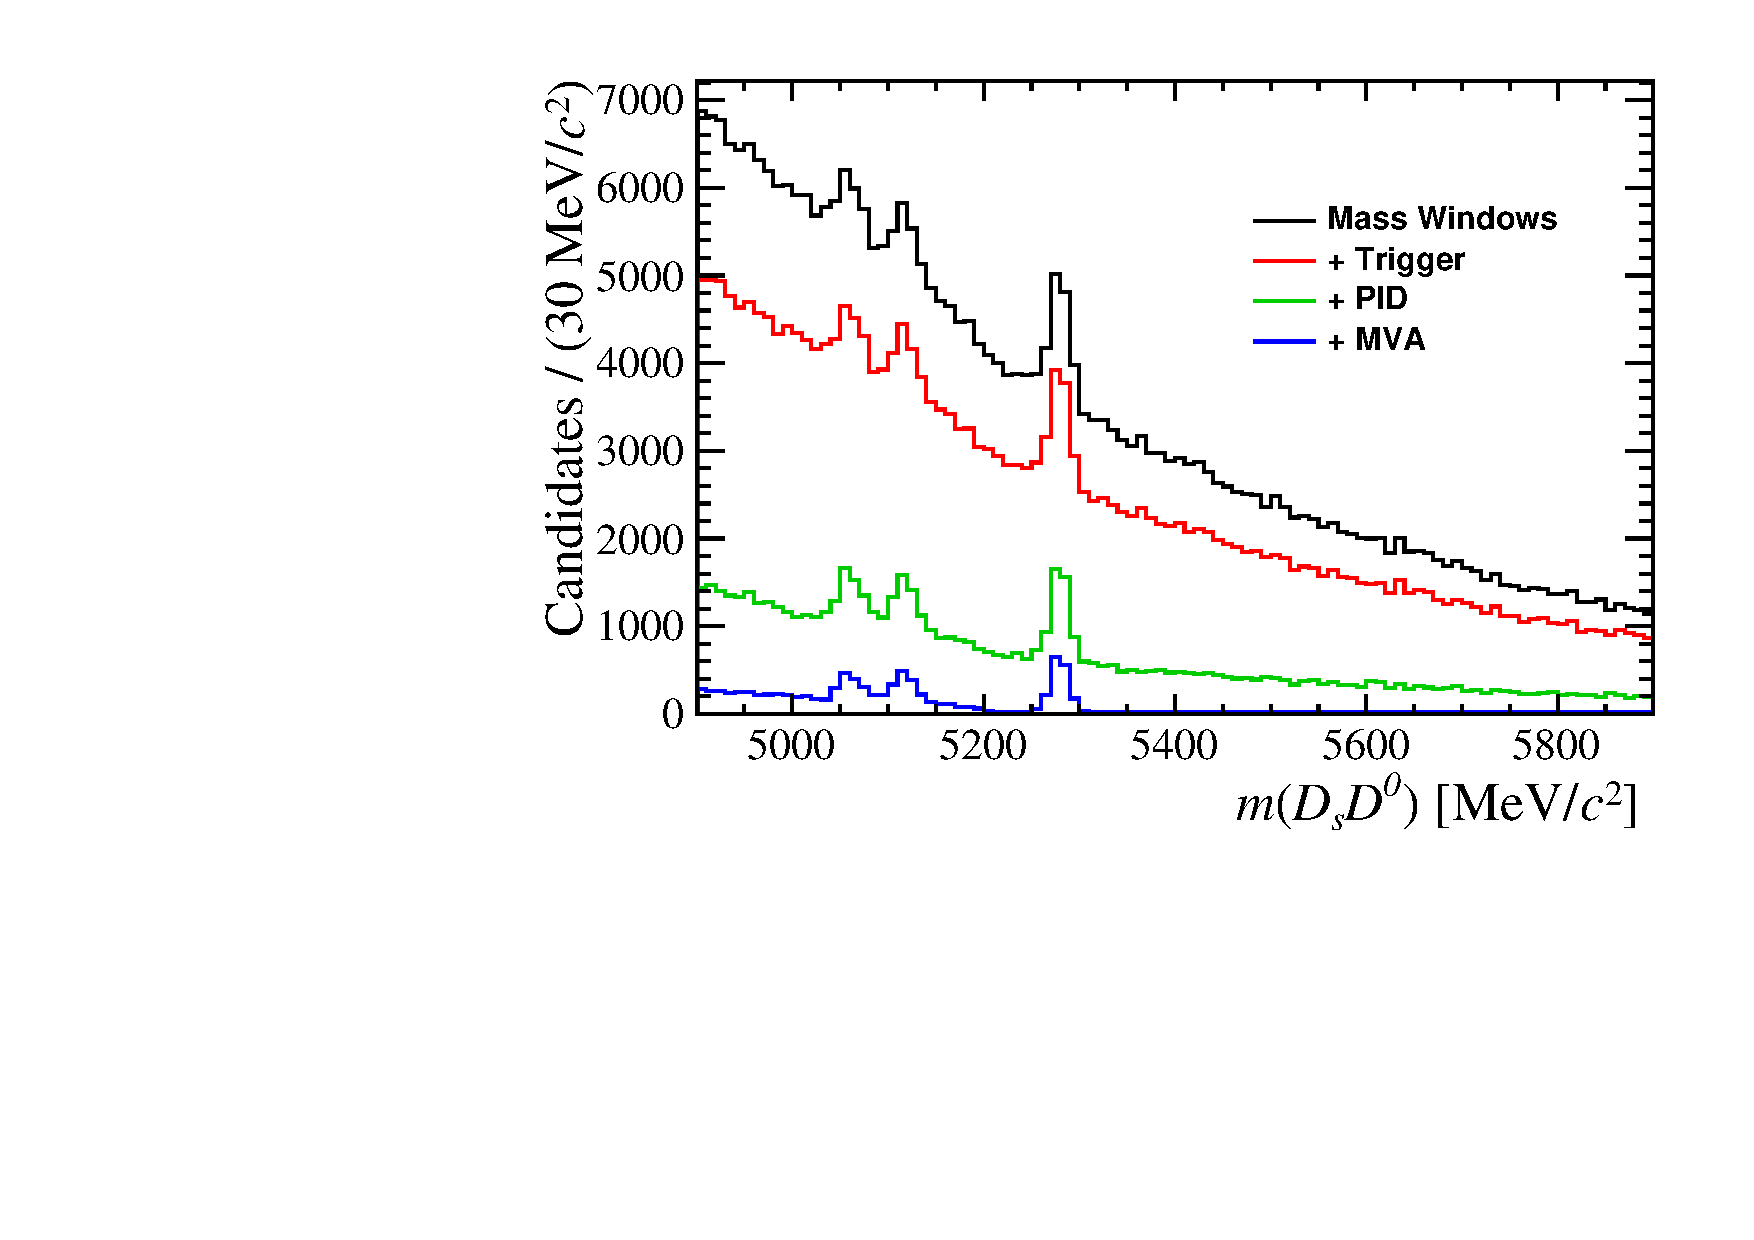
\includegraphics[width=0.8\textwidth]{figs/Selection/Normalisation_with_sel_B2DsD0.pdf}
    \caption{Various selection steps applied to the normalisation channel.}
    \label{fig:norm_selection}   
\end{figure}
%%%%%%%%%%%%%%%%%%%%%%%%%%%%%%%%%%%%%%%%%%%%%%%%%%%%%%%%%%


